\documentclass[newPxFont,nosectionpage]{beamer}

\usetheme{sthlm}
\usepackage{amsmath,amssymb,bm}
\usepackage{graphicx}
\usepackage{booktabs}
\usepackage{ragged2e}
\usepackage{array}

\newcommand{\pkg}[1]{{\normalfont\fontseries{b}\selectfont #1}}
\let\proglang\textsf
\newcommand{\bbeta}{\bm{\beta}}
\newcommand{\bX}{\bm{X}}
\newcommand{\by}{\bm{y}}
\newcommand{\bzero}{\bm{0}}
\newcommand{\bI}{\bm{I}}
\newcommand{\bA}{\bm{A}}
\newcommand{\bbr}{\bm{r}}
\newcommand{\bz}{\bm{z}}
\newcommand{\ba}{\bm{a}}
\newcommand{\hbbeta}{\widehat{\bm{\beta}}}
\newcommand{\norm}[1]{\left\lVert #1 \right\rVert}
\newcommand{\argmin}{\operatorname*{arg\,min}}
\newcommand{\soft}[2]{\mathcal{S}_{#1}\!\left(#2\right)}
\newcommand{\sectiondivider}[2]{%
  {\setbeamercolor{background canvas}{bg=sthlmDarkGrey}%
  \begin{frame}[plain]
    \vfill
    {\color{white}\fontsize{24}{29}\selectfont #1\par}
    \vspace{0.6em}
    {\color{sthlmBlue}\large #2\par}
    \vfill
  \end{frame}}
}

\setbeamertemplate{navigation symbols}{}
\setbeamertemplate{bibliography item}{\insertbiblabel}
\setbeamertemplate{title page}{%
  \vbox{}\vfill
  {\fontsize{18}{21}\selectfont\color{sthlmDarkGrey}\inserttitle\par}
  \vspace{0.1em}
  {\large\color{sthlmBlue}\insertsubtitle\par}
  \vspace{0.25em}
  \begin{tikzpicture}\draw[sthlmDarkGrey] (0, 0) -- (\textwidth, 0);\end{tikzpicture}
  \vspace{0.35em}
  {\large\insertauthor\par}
  \vspace{0.2em}
  {\normalsize\insertinstitute\par}
  \vspace{0.2em}
  {\normalsize\color{sthlmBlue}\insertdate\par}
  \vfill
}
\setbeamertemplate{footline}{%
  \leavevmode\hbox{%
  \begin{beamercolorbox}[wd=.38\paperwidth,ht=2.45ex,dp=1ex,left]{author in head/foot}%
    \hspace{1.3em}\usebeamerfont{author in head/foot}Bahad{\i}r Y\"{u}zba\c{s}{\i}
  \end{beamercolorbox}%
  \begin{beamercolorbox}[wd=.42\paperwidth,ht=2.45ex,dp=1ex,center]{title in head/foot}%
    \usebeamerfont{title in head/foot}HDDA-XV | Istanbul
  \end{beamercolorbox}%
  \begin{beamercolorbox}[wd=.20\paperwidth,ht=2.45ex,dp=1ex,right]{date in head/foot}%
    \insertframenumber{} / \inserttotalframenumber\hspace{1.4em}
  \end{beamercolorbox}}%
  \vskip0pt%
}

\title[A hybrid regularization framework]{A Hybrid Regularization Framework\\for Correlated Feature Selection\\in High-Dimensional Data}
\subtitle{Scaled Group Lasso (SGLASSO)}
\author[Bahad{\i}r Y\"{u}zba\c{s}{\i}]{Bahad{\i}r Y\"{u}zba\c{s}{\i}, PhD\\[0.35em]\small Joint work with Jiguo Cao}
\institute{Department of Econometrics\\\.{I}n\"{o}n\"{u} University, T\"{u}rkiye}
\date{HDDA-XV, Istanbul Medipol University\\12 August 2026}

\begin{document}

\maketitle

\begin{frame}{Talk roadmap}
\small
\begin{columns}[T,onlytextwidth]
\column{0.48\textwidth}
\begin{block}{Problem and method}
\begin{enumerate}
  \item Why grouped high-dimensional predictors are difficult under collinearity.
  \item How SGLASSO modifies the usual group-penalty shrinkage target.
  \item How the block-coordinate solver fits the path efficiently.
\end{enumerate}
\end{block}
\column{0.48\textwidth}
\begin{block}{Evidence and interpretation}
\begin{enumerate}
  \item Simulation evidence on prediction, recovery, selection, and runtime.
  \item GenAtHum gene-expression application with tissue/cell-type groups.
  \item Practical take-home messages for grouped data analysis.
\end{enumerate}
\end{block}
\end{columns}
\end{frame}

\sectiondivider{1. Motivation}{Known groups, correlated predictors, and a prediction--sparsity trade-off}

\begin{frame}{Why correlated groups make selection difficult}
\begin{columns}[T,onlytextwidth]
\column{0.56\textwidth}
\scriptsize
High-dimensional predictors often arrive with a known group structure: pathways, basis expansions, tissues, or related sensors.

\vspace{0.25em}
\begin{itemize}
  \item \textbf{Featurewise selection} can fragment a meaningful group.
  \item \textbf{Groupwise selection} respects structure, but correlation makes overlapping groups hard to separate.
  \item \textbf{Prediction tuning} can retain related groups when they improve out-of-sample error.
\end{itemize}

\vspace{0.1em}
\textbf{Question:} can group sparsity and stable estimation coexist under collinearity?
\column{0.40\textwidth}
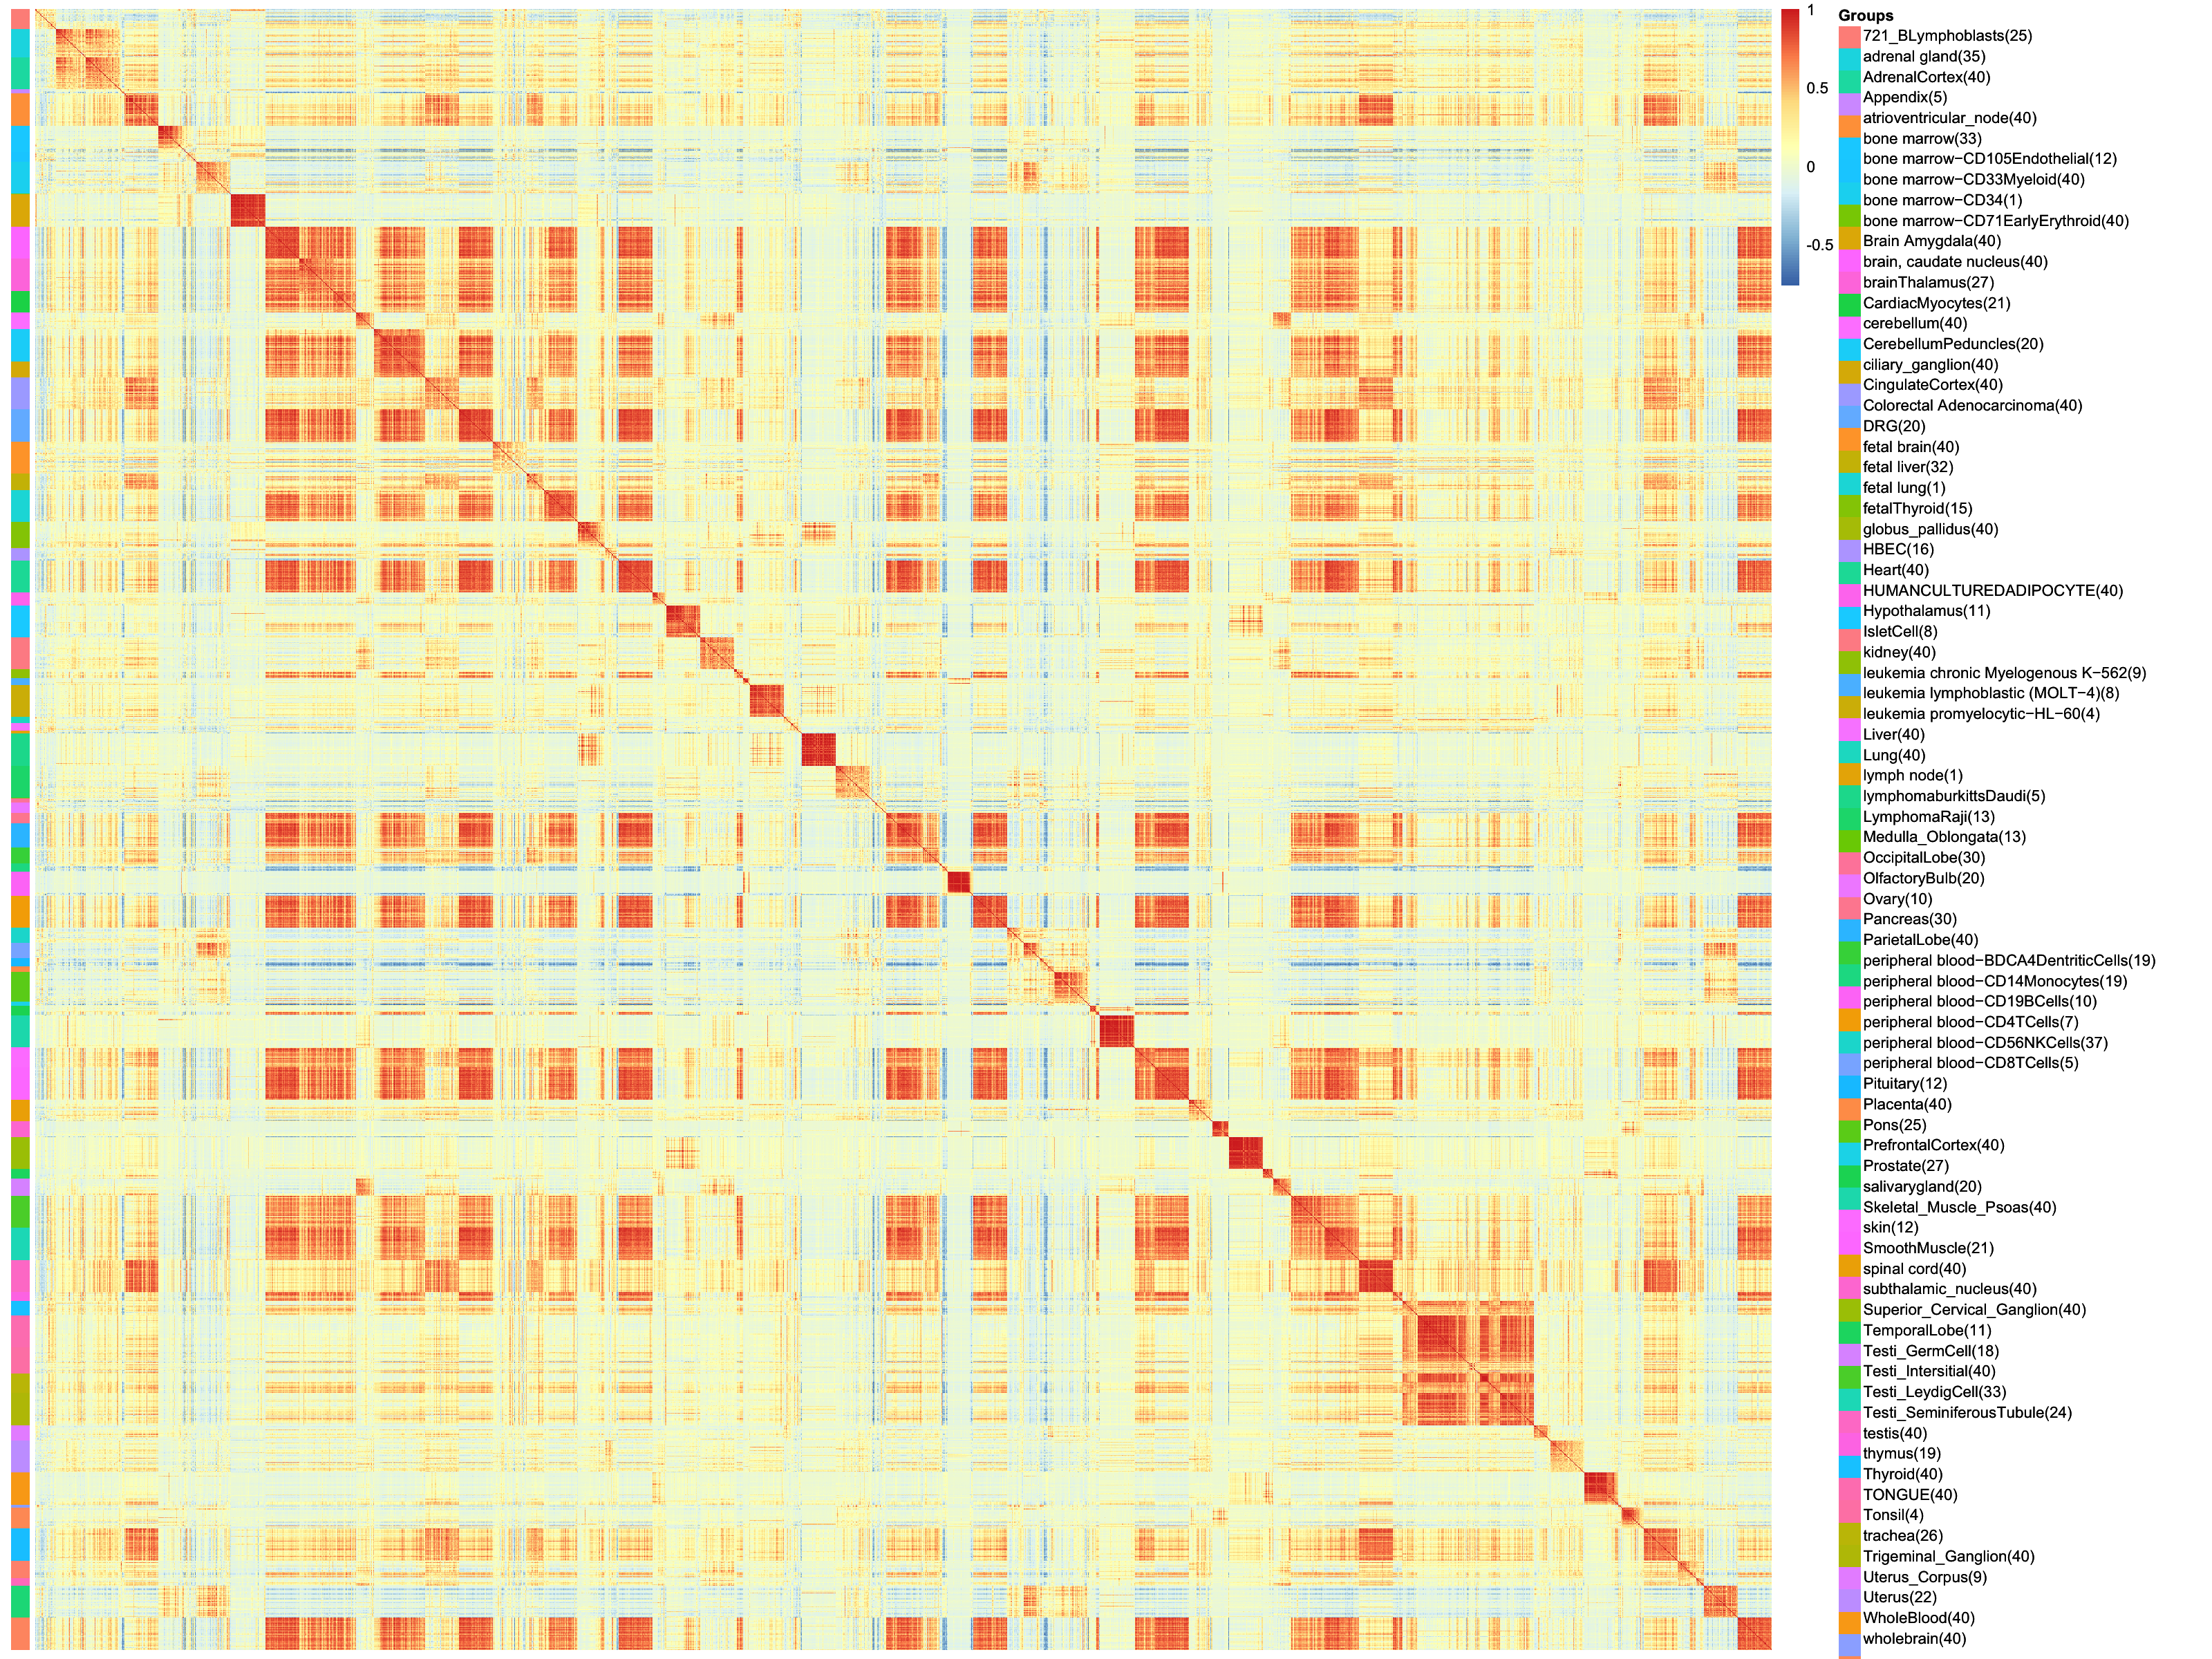
\includegraphics[width=\linewidth]{pheatmat_gene.png}
\end{columns}
\end{frame}

\begin{frame}{What changes in grouped high-dimensional data?}
\small
\begin{columns}[T,onlytextwidth]
\column{0.31\textwidth}
\begin{block}{Structure}
Predictors are not isolated: genes, tissues, pathways, basis functions, and repeated measurements naturally form groups.
\end{block}
\column{0.31\textwidth}
\begin{block}{Collinearity}
Groups can carry similar signal. Removing one correlated group may improve sparsity but hurt prediction or coefficient recovery.
\end{block}
\column{0.31\textwidth}
\begin{block}{Tuning}
Validation-based tuning often favors prediction, so the selected model may be broader than the sparsest scientifically plausible model.
\end{block}
\end{columns}
\vspace{0.55em}
\begin{alertblock}{Design goal}
SGLASSO is designed as a flexible regularization point between pure group sparsity and shrinkage toward a data-informed target.
\end{alertblock}
\end{frame}

\sectiondivider{2. Scaled Group Lasso}{A groupwise penalty with a data-informed shrinkage target}

\begin{frame}{A grouped linear model}
\Large
\[
  \by = \beta_0\bm{1} + \sum_{j=1}^{J}\bX_j\bbeta_j + \bm{\varepsilon},
  \qquad \bm{\varepsilon}\sim N(\bzero,\sigma^2\bI).
\]
\normalsize

\begin{columns}[T,onlytextwidth]
\column{0.48\textwidth}
\begin{block}{What is selected?}
Each $\bbeta_j\in\mathbb{R}^{p_j}$ is a block of coefficients. A groupwise method either keeps or removes the block as a unit.
\end{block}
\column{0.48\textwidth}
\begin{block}{Why is it difficult?}
When $\bX_j$ and $\bX_\ell$ are correlated, several groups can carry overlapping signal. Aggressive selection may discard useful information.
\end{block}
\end{columns}

\vspace{0.35em}
\small
%The group lasso induces group sparsity through $\lambda\sum_{j=1}^{J}\sqrt{p_j}\norm{\bbeta_j}_2$ \citep{yuan2006model}.
\end{frame}

\begin{frame}{Group Lasso is the starting point}
\small
\[
  \widehat{\bbeta}^{\rm GL}=
  \argmin_{\bbeta}\left\{
  \frac{1}{2n}\norm{\by-\bX\bbeta}_2^2+
  \lambda\sum_{j=1}^{J}w_j\norm{\bbeta_j}_2\right\},
  \qquad w_j=\sqrt{M_j}.
\]
\begin{columns}[T,onlytextwidth]
\column{0.30\textwidth}
\begin{block}{Key idea}
Select or remove a whole coefficient block.
\end{block}
\column{0.30\textwidth}
\begin{block}{Why it matters}
Scientific grouping is used directly rather than ignored.
\end{block}
\column{0.30\textwidth}
\begin{block}{Open issue}
All selected groups are shrunk toward zero, even when groups are correlated.
\end{block}
\end{columns}
\vspace{0.35em}
\small\centering
\scriptsize SGLASSO retains Group Lasso's selection rule and changes the shrinkage target for correlated groups \citep{yuan2006model}.
\end{frame}

\begin{frame}{The modeling move: change the shrinkage target}
\small
\begin{center}
\renewcommand{\arraystretch}{1.45}
\begin{tabular}{>{\bfseries}l p{0.32\textwidth} p{0.32\textwidth}}
\toprule
Method & Group sparsity & Quadratic shrinkage target \\
\midrule
Group Lasso & Yes & None \\
Group elastic net & Yes & $\bm{0}$ \\
SGLASSO & Yes & $d\widehat{\bbeta}^{\rm LSE}_j$ \\
\bottomrule
\end{tabular}
\end{center}
\vspace{0.8em}
\begin{block}{Interpretation}
The target preserves group selection while modifying the shrinkage destination. The parameter $d$ controls its influence \citep{zou2005regularization,helwig2024versatile,james1961estimation,arashi2021slasso}.
\end{block}
\end{frame}

\begin{frame}{Why a scaled target can help}
\small
\begin{columns}[T,onlytextwidth]
\column{0.48\textwidth}
\begin{block}{Zero-centered shrinkage}
Group Lasso and group elastic net pull selected coefficients toward zero. This is effective for sparsity, but can be too aggressive when correlated groups share signal.
\end{block}
\column{0.48\textwidth}
\begin{block}{SGLASSO shrinkage}
The quadratic part pulls group $j$ toward $d\widehat{\bbeta}^{\rm LSE}_j$. This keeps the groupwise selection mechanism but allows a nonzero shrinkage target.
\end{block}
\end{columns}
\vspace{0.45em}
\begin{alertblock}{Role of $d$}
The scale parameter does not create a new grouping structure; it changes how strongly the selected group is pulled toward the least-squares-based direction.
\end{alertblock}
\end{frame}

\begin{frame}{SGLASSO combines group sparsity and scaled shrinkage}
\small
\[
\widehat{\bbeta} = \argmin_{\bbeta\in\mathbb{R}^p}
\left\{\begin{aligned}
&\frac{1}{2n}\norm{\by-\bX\bbeta}_2^2
+ \lambda\alpha\sum_{j=1}^{J} w_j\norm{\bbeta_j}_2\\
&+\frac{\lambda(1-\alpha)}{2}\sum_{j=1}^{J}w_j
\norm{\bbeta_j-d\widehat{\bbeta}^{\rm LSE}_j}_2^2
\end{aligned}\right\},
\qquad w_j=\sqrt{M_j},
\]

\begin{columns}[T,onlytextwidth]
\column{0.31\textwidth}
\begin{block}{$\lambda$}
Overall regularization level.
\end{block}
\column{0.31\textwidth}
\begin{block}{$\alpha$}
Balances group sparsity and quadratic shrinkage.
\end{block}
\column{0.31\textwidth}
\begin{block}{$d$}
Sets the scaled least-squares target.
\end{block}
\end{columns}

\vspace{0.25em}
\small Here $M_j$ is the number of predictors in group $j$. When $\alpha=1$, the quadratic term vanishes and SGLASSO reduces to group lasso.
\end{frame}

\begin{frame}{The scale parameter changes the shrinkage target}
\begin{columns}[c,onlytextwidth]
\column{0.72\textwidth}
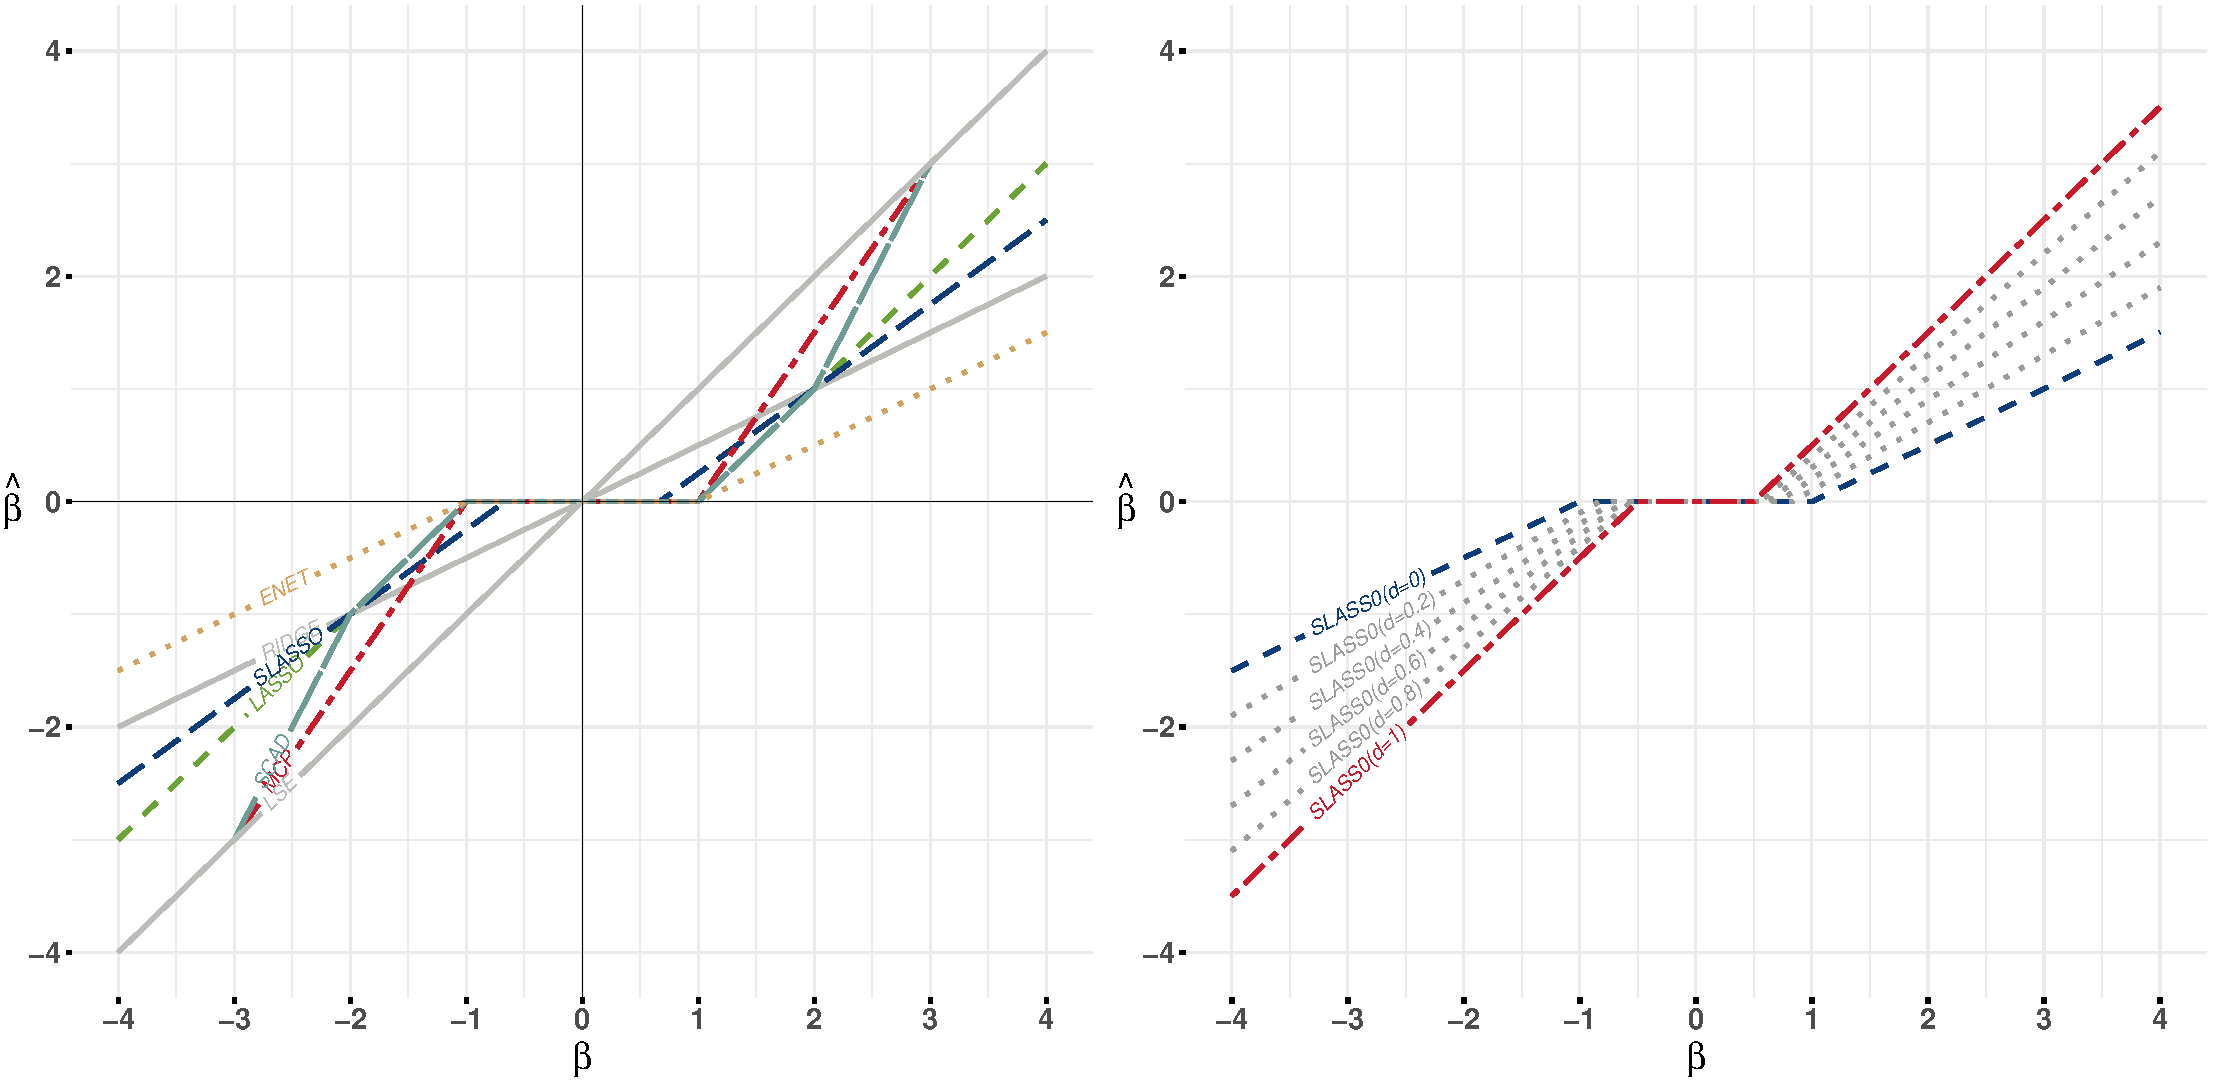
\includegraphics[width=\linewidth]{pen_sol_plots.pdf}
\column{0.24\textwidth}
\scriptsize
\begin{block}{Interpretation}
Quadratic shrinkage targets $d\widehat{\bbeta}_j^{\rm LSE}$, not only zero.
\end{block}
\vspace{0.25em}
\textbf{$d=0$:} zero-centered quadratic shrinkage.\medskip
\textbf{$0<d<1$:} an intermediate, scaled target.\medskip
\textbf{$d=1$:} the full group-LSE target.
\end{columns}
\end{frame}

\begin{frame}{From the objective to one block subproblem}
\footnotesize
After standardization and group orthonormalization, hold all blocks except $j$ fixed. Let
\[
  \bz_j=\frac{1}{n}\bX_j^\top\bbr+\bbeta_j,
  \qquad
  \bA_j=\bz_j+\lambda_2w_jd\widehat{\bbeta}^{\rm LSE}_j,
  \quad \lambda_1=\lambda\alpha,\ \lambda_2=\lambda(1-\alpha).
\]
The block update minimizes, up to a constant,
\[
  \frac{1+\lambda_2w_j}{2}
  \left\lVert\bbeta_j-\frac{\bA_j}{1+\lambda_2w_j}\right\rVert_2^2
  +\lambda_1w_j\norm{\bbeta_j}_2.
\]
\begin{columns}[T,onlytextwidth]
\column{0.46\textwidth}
\begin{block}{What enters $\bA_j$?}
The partial residual score, the current block coefficient, and the scaled least-squares target.
\end{block}
\column{0.46\textwidth}
\begin{block}{Why this is useful}
The multivariate block problem reduces to one proximal group-thresholding operation.
\end{block}
\end{columns}
\vspace{0.25em}
\scriptsize This is the groupwise analogue of a coordinate-descent subproblem \citep{yuan2006model,breheny2015group}.
\end{frame}

\begin{frame}{KKT conditions give two groupwise cases}
\small
The blockwise KKT condition is
\[
  \bm{0}\in(1+\lambda_2w_j)\widehat{\bbeta}_j-\bA_j+
  \lambda_1w_j\,\partial\norm{\widehat{\bbeta}_j}_2.
\]
\begin{columns}[T,onlytextwidth]
\column{0.48\textwidth}
\begin{block}{Case 1: inactive group}
At $\widehat{\bbeta}_j=\bzero$, the subgradient has norm at most one. Therefore,
\[
\norm{\bA_j}_2\leq\lambda_1w_j
\quad\Rightarrow\quad\widehat{\bbeta}_j=\bzero.
\]
\end{block}
\column{0.48\textwidth}
\begin{block}{Case 2: active group}
When $\norm{\bA_j}_2>\lambda_1w_j$, the solution is aligned with $\bA_j$ and is shrunk as a vector.
\end{block}
\end{columns}
\end{frame}

\begin{frame}{Group soft-thresholding is the BCD update}
\footnotesize
Define the vector soft-thresholding operator
\[
  \soft{\tau}{\ba}=
  \left(1-\frac{\tau}{\norm{\ba}_2}\right)_+\ba,
  \qquad \ba\in\mathbb{R}^{M_j}.
\]
Then the exact update is
\[
  \widehat{\bbeta}_j=
  \frac{1}{1+\lambda_2w_j}\,
  \soft{\lambda_1w_j}{\bA_j}.
\]
\begin{columns}[T,onlytextwidth]
\column{0.47\textwidth}
\begin{block}{Selection and shrinkage are distinct}
The operator selects the whole group; the denominator applies quadratic shrinkage afterward.
\end{block}
\column{0.47\textwidth}
\begin{block}{Residual update}
Use $\bbr\leftarrow\bbr-\bX_j(\bbeta_j^{\rm new}-\bbeta_j)$ after each block. No full $\bX\bbeta$ recomputation is needed.
\end{block}
\end{columns}
\vspace{0.35em}
\scriptsize The formula remains valid for unequal group sizes through $w_j=\sqrt{M_j}$.
\end{frame}

\begin{frame}{Pathwise SSR: screen first, verify exactly}
\scriptsize
At the previous path point $\lambda^{(k)}$, SGLASSO uses the score
\[
G_j^{(k)}=\left\lVert
\frac{1}{n}\bX_j^\top\bbr(\lambda^{(k)})+
\lambda^{(k)}(1-\alpha)w_j
\left\{d\widehat{\bbeta}^{\rm LSE}_j-\widehat{\bbeta}_j(\lambda^{(k)})\right\}
\right\rVert_2.
\]
SSR discards a currently inactive group for $\lambda^{(k+1)}$ when
\[
  G_j^{(k)}<\alpha w_j\left(2\lambda^{(k+1)}-\lambda^{(k)}\right).
\]
\begin{columns}[T,onlytextwidth]
\column{0.47\textwidth}
\begin{block}{Fast candidate reduction}
Fit from large to small $\lambda$, warm-starting from the preceding solution and updating only the retained working set.
\end{block}
\column{0.47\textwidth}
\begin{block}{KKT verification}
SSR is strong, not safe. Check $G_j(\lambda^{(k+1)})\leq\alpha w_j\lambda^{(k+1)}$; restore and refit any violation.
\end{block}
\end{columns}
\vspace{0.2em}
\scriptsize The shifted term is specific to SGLASSO; final KKT checks recover the exact fitted path \citep{friedman2007pathwise,tibshirani2012strong}.
\end{frame}

\begin{frame}{Solver workflow}
\footnotesize
\begin{columns}[T,onlytextwidth]
\column{0.47\textwidth}
\begin{block}{Preparation}
\begin{enumerate}
  \item Standardize predictors.
  \item Orthonormalize each group.
  \item Build a decreasing $\lambda$ path.
  \item Initialize with the previous path solution.
\end{enumerate}
\end{block}
\column{0.47\textwidth}
\begin{block}{Path fitting}
\begin{enumerate}
  \item Apply SSR to remove unlikely inactive groups.
  \item Cycle through active/working groups by BCD.
  \item Update residuals incrementally.
  \item Check final KKT conditions and refit if needed.
\end{enumerate}
\end{block}
\end{columns}
\vspace{0.25em}
\centering\scriptsize\color{sthlmBlue}
Computational message: reduce repeated full-design calculations while retaining final KKT verification.
\end{frame}

\sectiondivider{3. Simulation evidence}{Prediction, recovery, selection, and computational scaling}

\begin{frame}{Simulation design: a controlled correlation experiment}
\begin{columns}[T,onlytextwidth]
\column{0.48\textwidth}
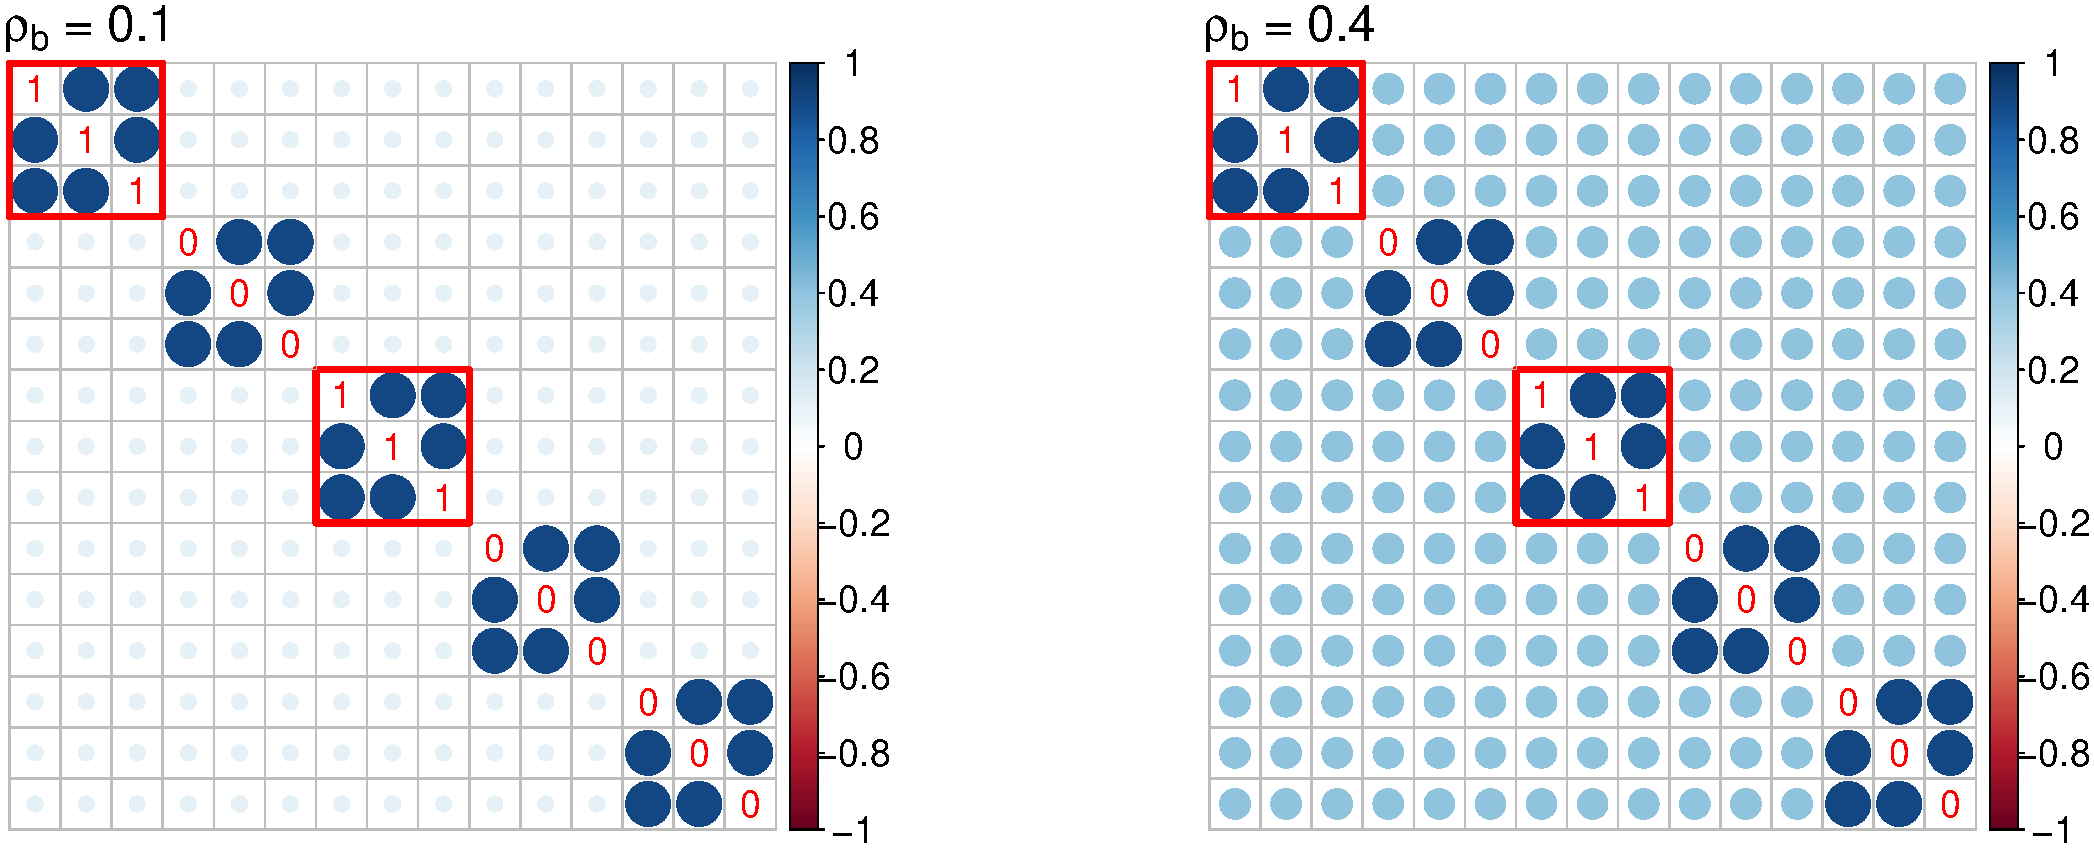
\includegraphics[width=\linewidth]{sim_data_LD.pdf}
\column{0.47\textwidth}
\scriptsize
\begin{block}{Grouped Gaussian design}
HD settings: $n=100$, $p=1000$, $J=200$\\
Five predictors per group; $s\in\{10,20,40\}$ active groups.\\
Within-group correlation: $\rho_w=0.9$; between-group correlation: $\rho_b\in\{0,0.1,\ldots,0.9\}$.\\
SNR: $0.05$ to $6$; tuning is by validation prediction error.
\end{block}
\begin{block}{Signal patterns}
\textbf{Homogeneous:} common active magnitude.\\
\textbf{Weak/strong mixed:} two active magnitudes.
\end{block}
\end{columns}
\end{frame}

\begin{frame}{Competing methods}
\footnotesize
\begin{columns}[T,onlytextwidth]
\column{0.48\textwidth}
\begin{block}{Grouped BCD-type estimators}
\begin{itemize}
  \item GLASSO: group sparsity.
  \item GSCAD and GMCP: nonconvex group penalties.
  \item GENET: group elastic-net regularization.
  \item SGLASSO: group sparsity plus scaled shrinkage.
\end{itemize}
\end{block}
\column{0.48\textwidth}
\begin{block}{Specialized baseline}
ADELIE is included as a modern high-speed grouped-regularization benchmark.
\end{block}
\begin{block}{Fair comparison principle}
Methods use common training, validation, and test samples.
\end{block}
\end{columns}
\end{frame}

\begin{frame}{Read the simulation results as a multi-criterion comparison}
\footnotesize
\begin{columns}[T,onlytextwidth]
\column{0.48\textwidth}
\begin{block}{Prediction and estimation}
\textbf{Test MSE.} Out-of-sample squared prediction error.\par\smallskip
\textbf{Coefficient MSE.} Squared error in recovering $\bbeta$.\par\smallskip
\textbf{PVE.} Proportion of signal variation explained.
\end{block}
\column{0.48\textwidth}
\begin{block}{Selection and computation}
\textbf{FDR.} False discoveries among selected terms.\par\smallskip
\textbf{$\widehat{s}$.} Number of selected groups.\par\smallskip
\textbf{Runtime.} Serial fitting time over a regularization path.
\end{block}
\end{columns}
\vspace{0.25em}
\begin{alertblock}{Interpretation principle}
No single criterion fully characterizes a grouped estimator: validation-MSE tuning can favor a broader model if correlated groups improve prediction.
\end{alertblock}
\end{frame}

\begin{frame}{Prediction under correlation}
\begin{figure}
\centering
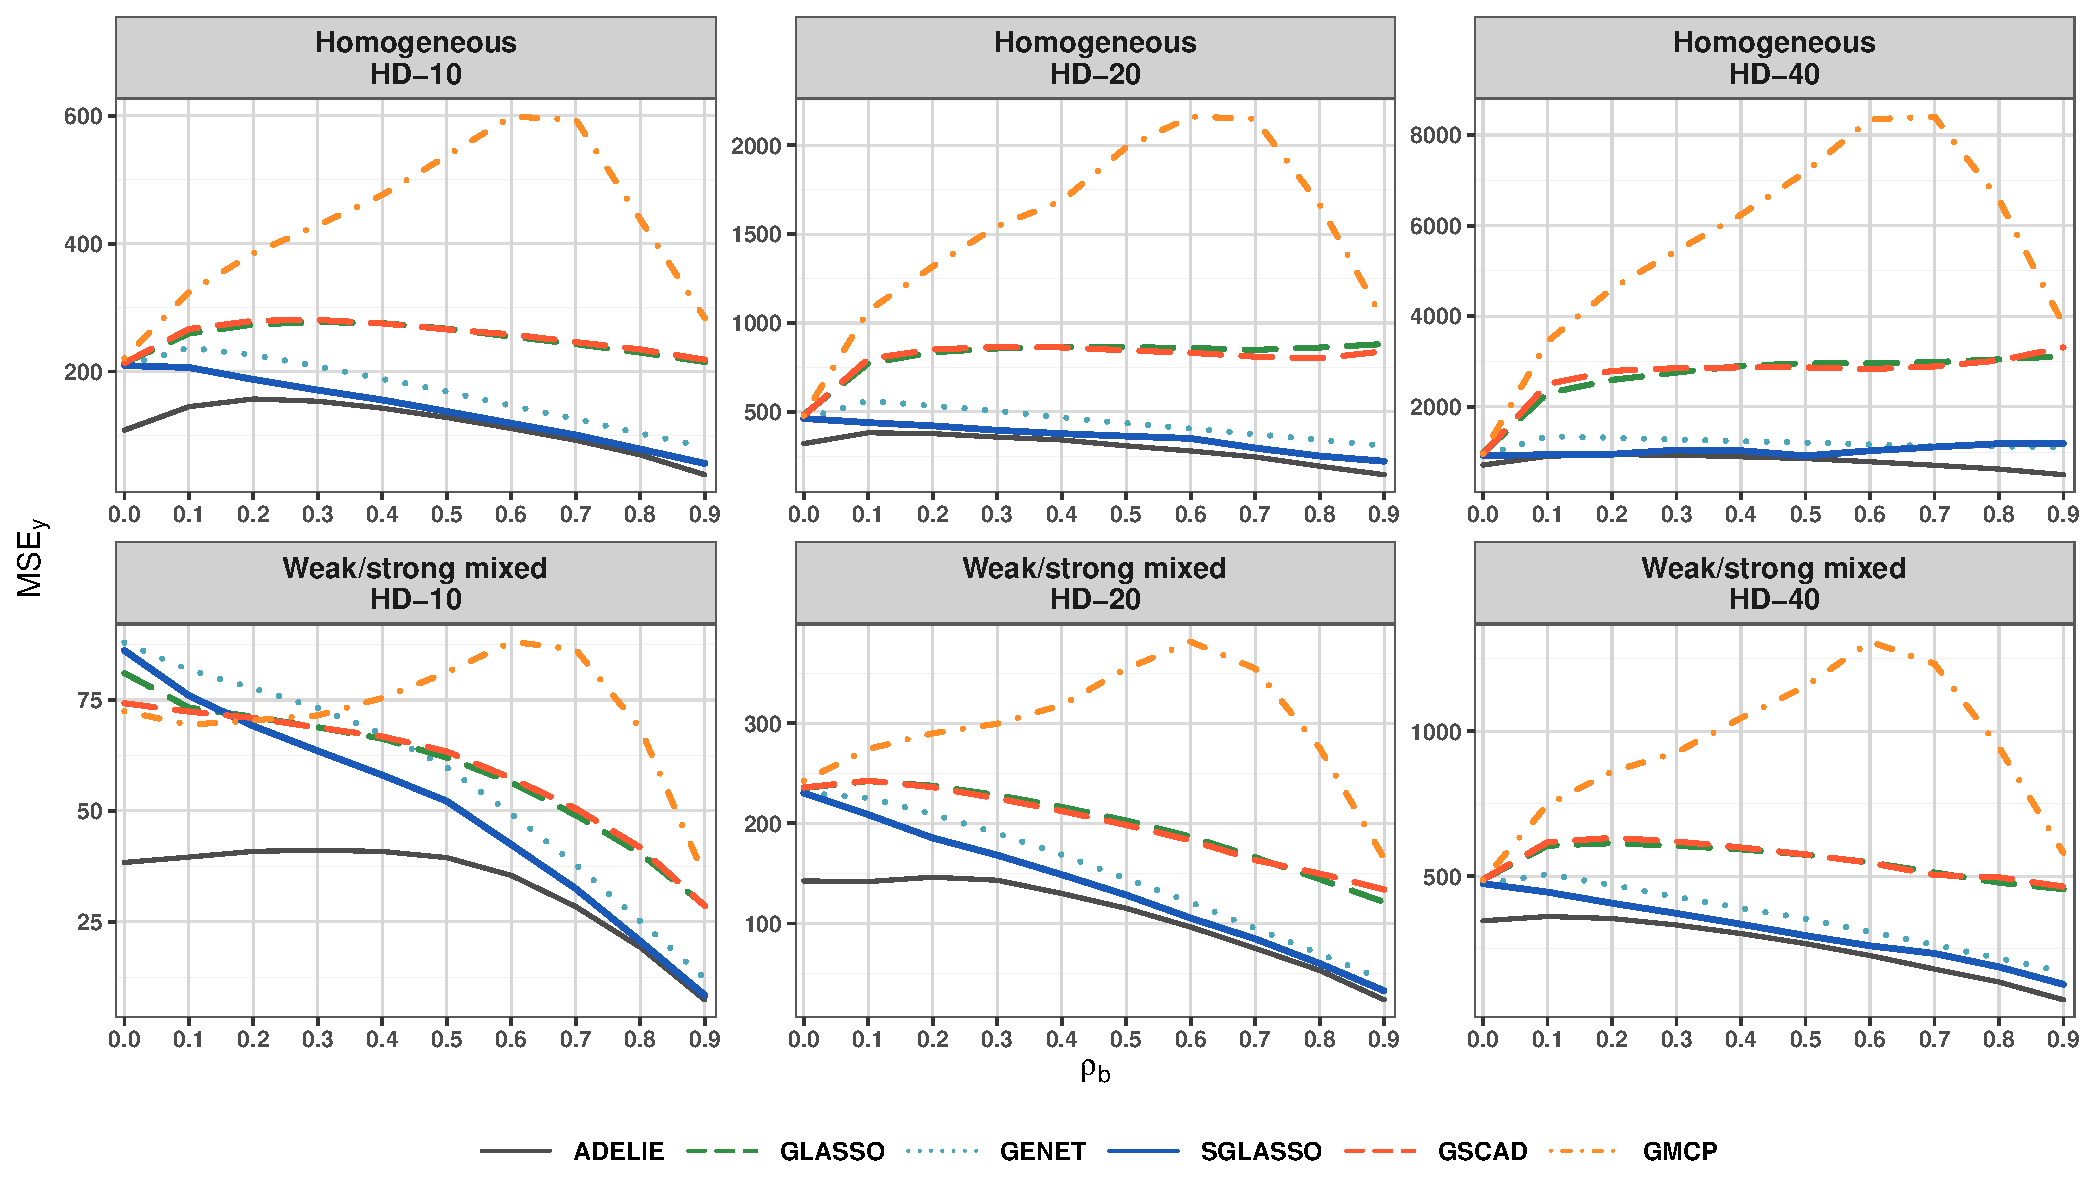
\includegraphics[height=0.64\textheight,keepaspectratio]{main_sim_HD_mse_y_vs_rhob.pdf}
\end{figure}
\vspace{-0.45em}
\scriptsize
HD: $p=1000$, $J=200$, $\mathrm{SNR}=1.528$. SGLASSO remains close to the best predictive methods as between-group correlation increases.
\end{frame}

\begin{frame}{Coefficient recovery under correlation}
\begin{figure}
\centering
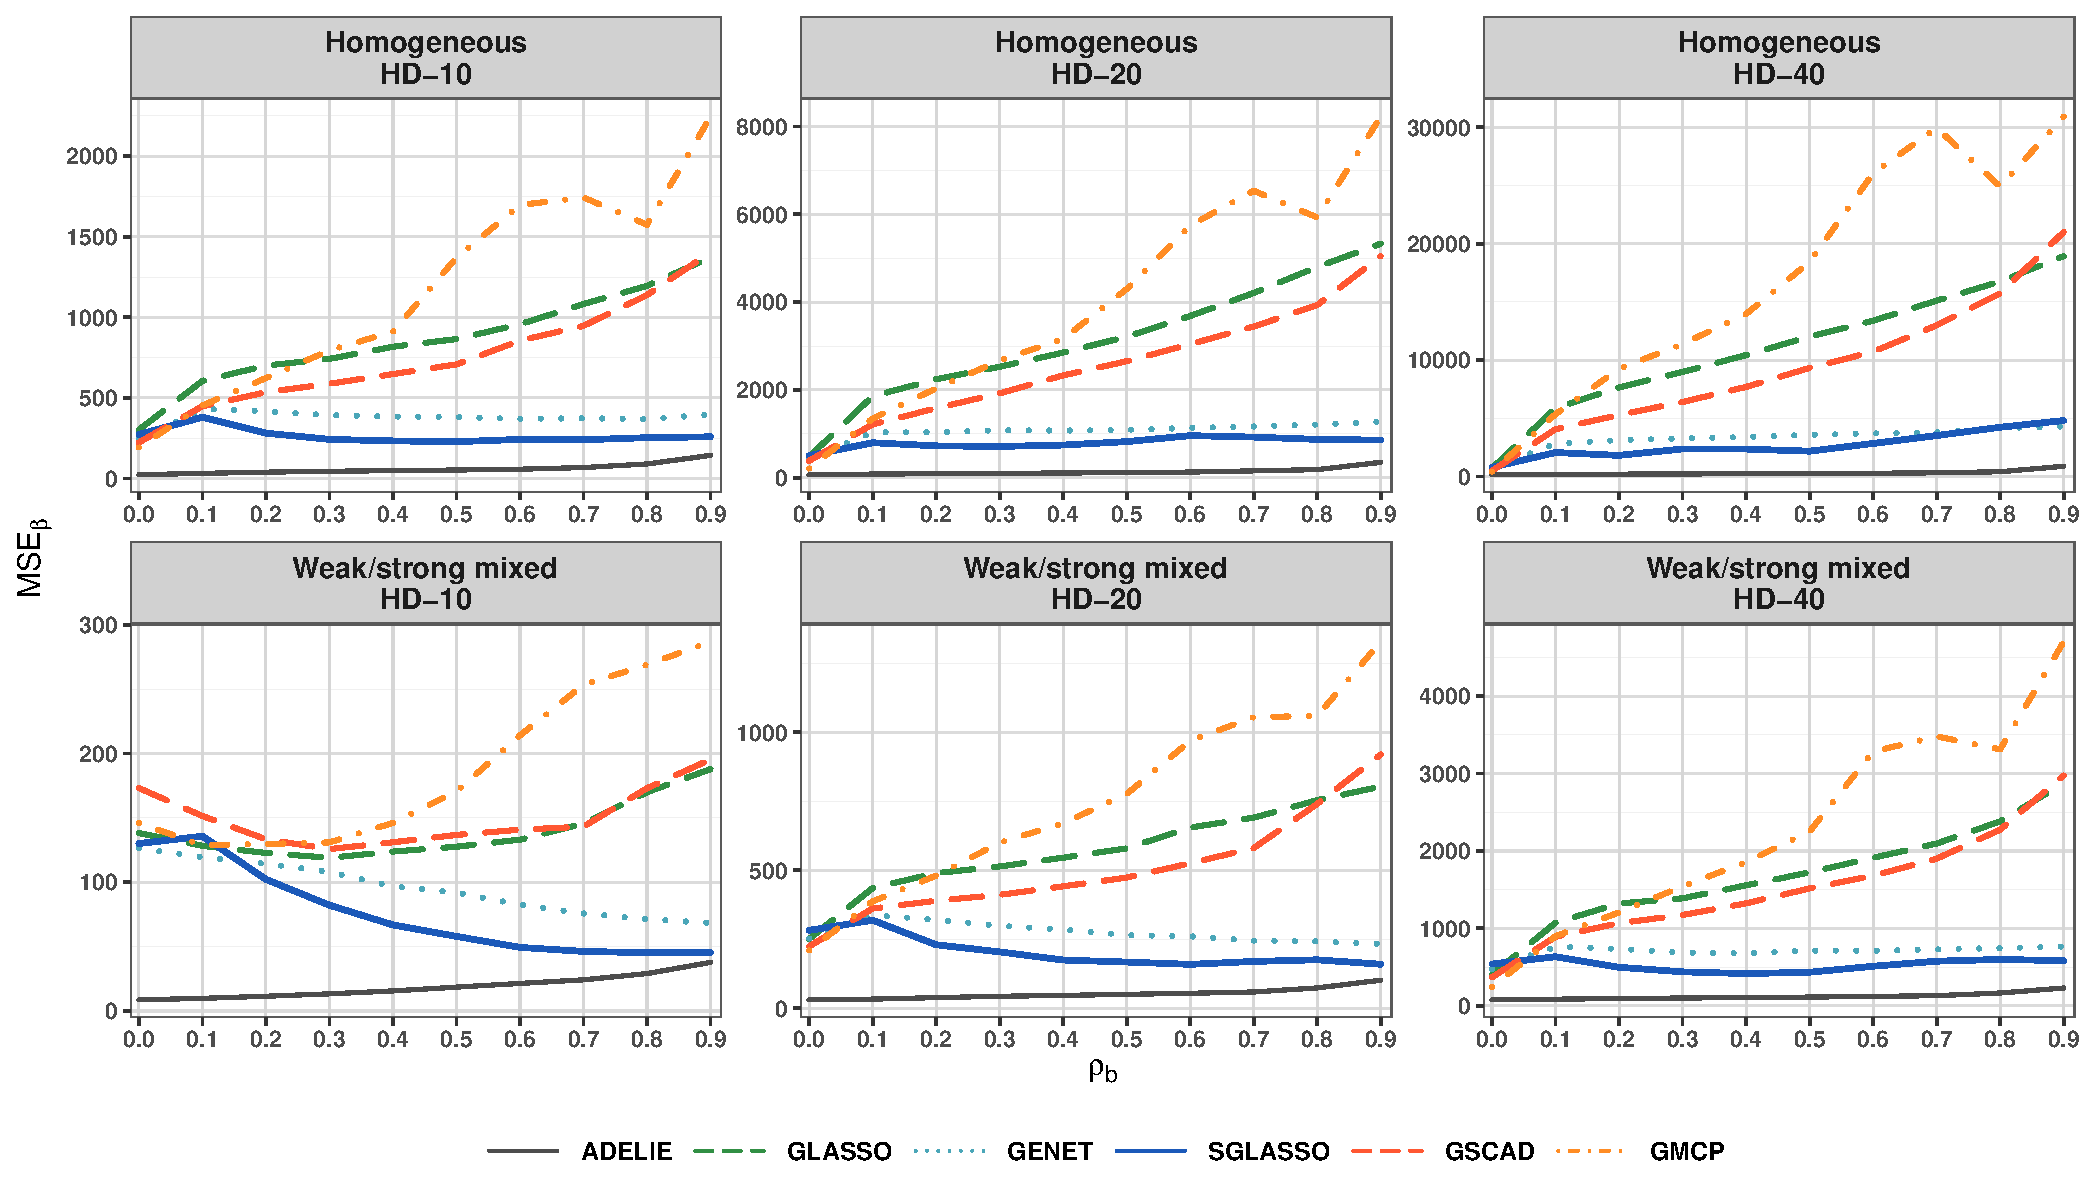
\includegraphics[height=0.64\textheight,keepaspectratio]{main_sim_HD_mse_beta_vs_rhob.pdf}
\end{figure}
\vspace{-0.45em}
\scriptsize
Coefficient MSE asks whether the fitted path recovers the grouped signal, not only whether it predicts well.
\end{frame}

\begin{frame}{PVE improves with signal strength}
\begin{figure}
\centering
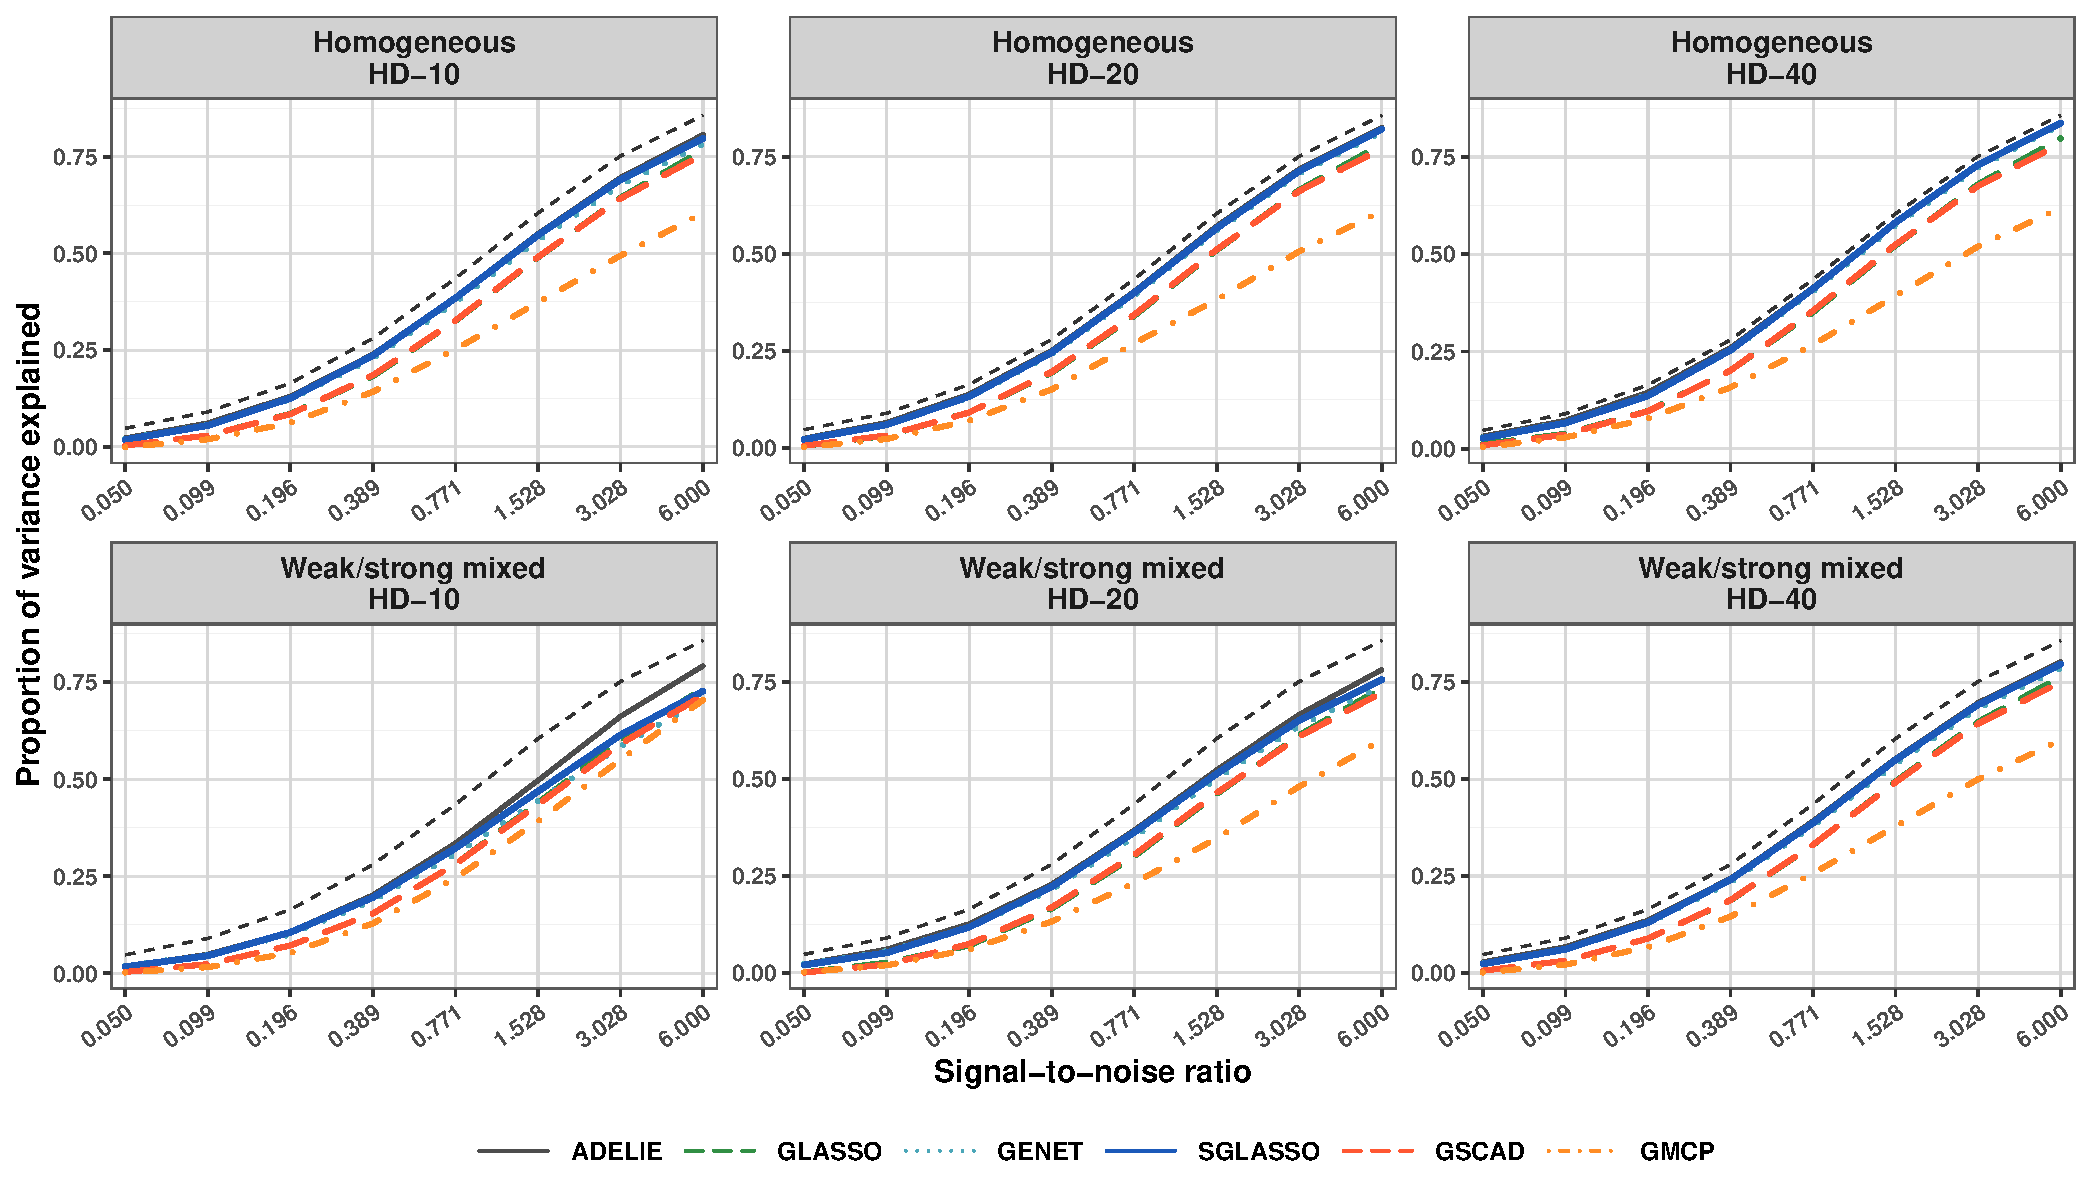
\includegraphics[height=0.64\textheight,keepaspectratio]{main_sim_HD_pve_vs_snr.pdf}
\end{figure}
\vspace{-0.45em}
\scriptsize PVE increases with SNR. The dashed curve is $\mathrm{SNR}/(1+\mathrm{SNR})$; SGLASSO tracks the leading predictive methods.
\end{frame}

\begin{frame}{Selection: prediction versus sparsity}
\begin{columns}[T,onlytextwidth]
\column{0.49\textwidth}
\centering
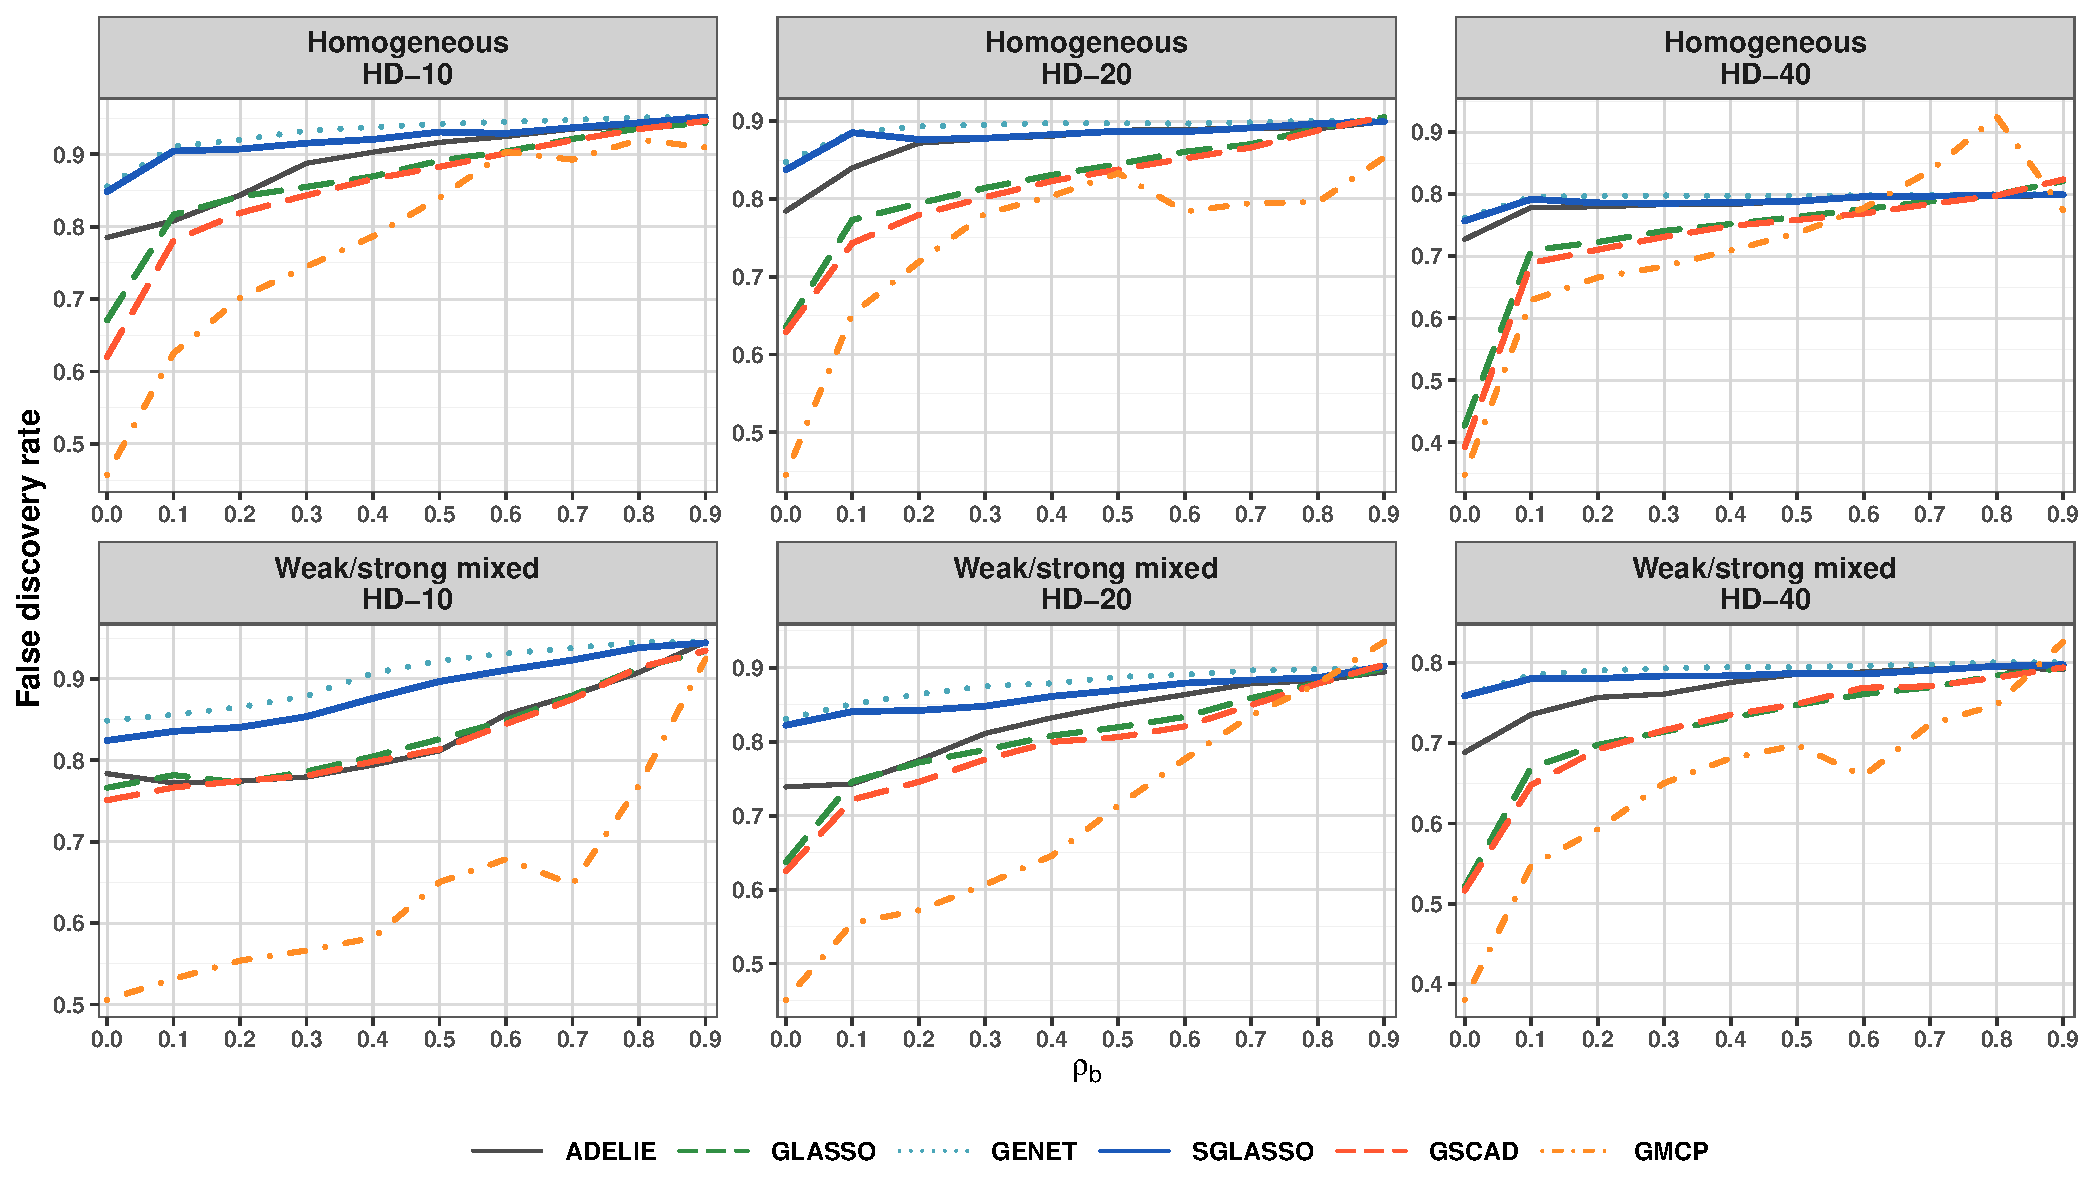
\includegraphics[width=\linewidth]{main_sim_HD_fdr_vs_rhob.pdf}\\[-0.25em]
\scriptsize False discovery rate
\column{0.49\textwidth}
\centering
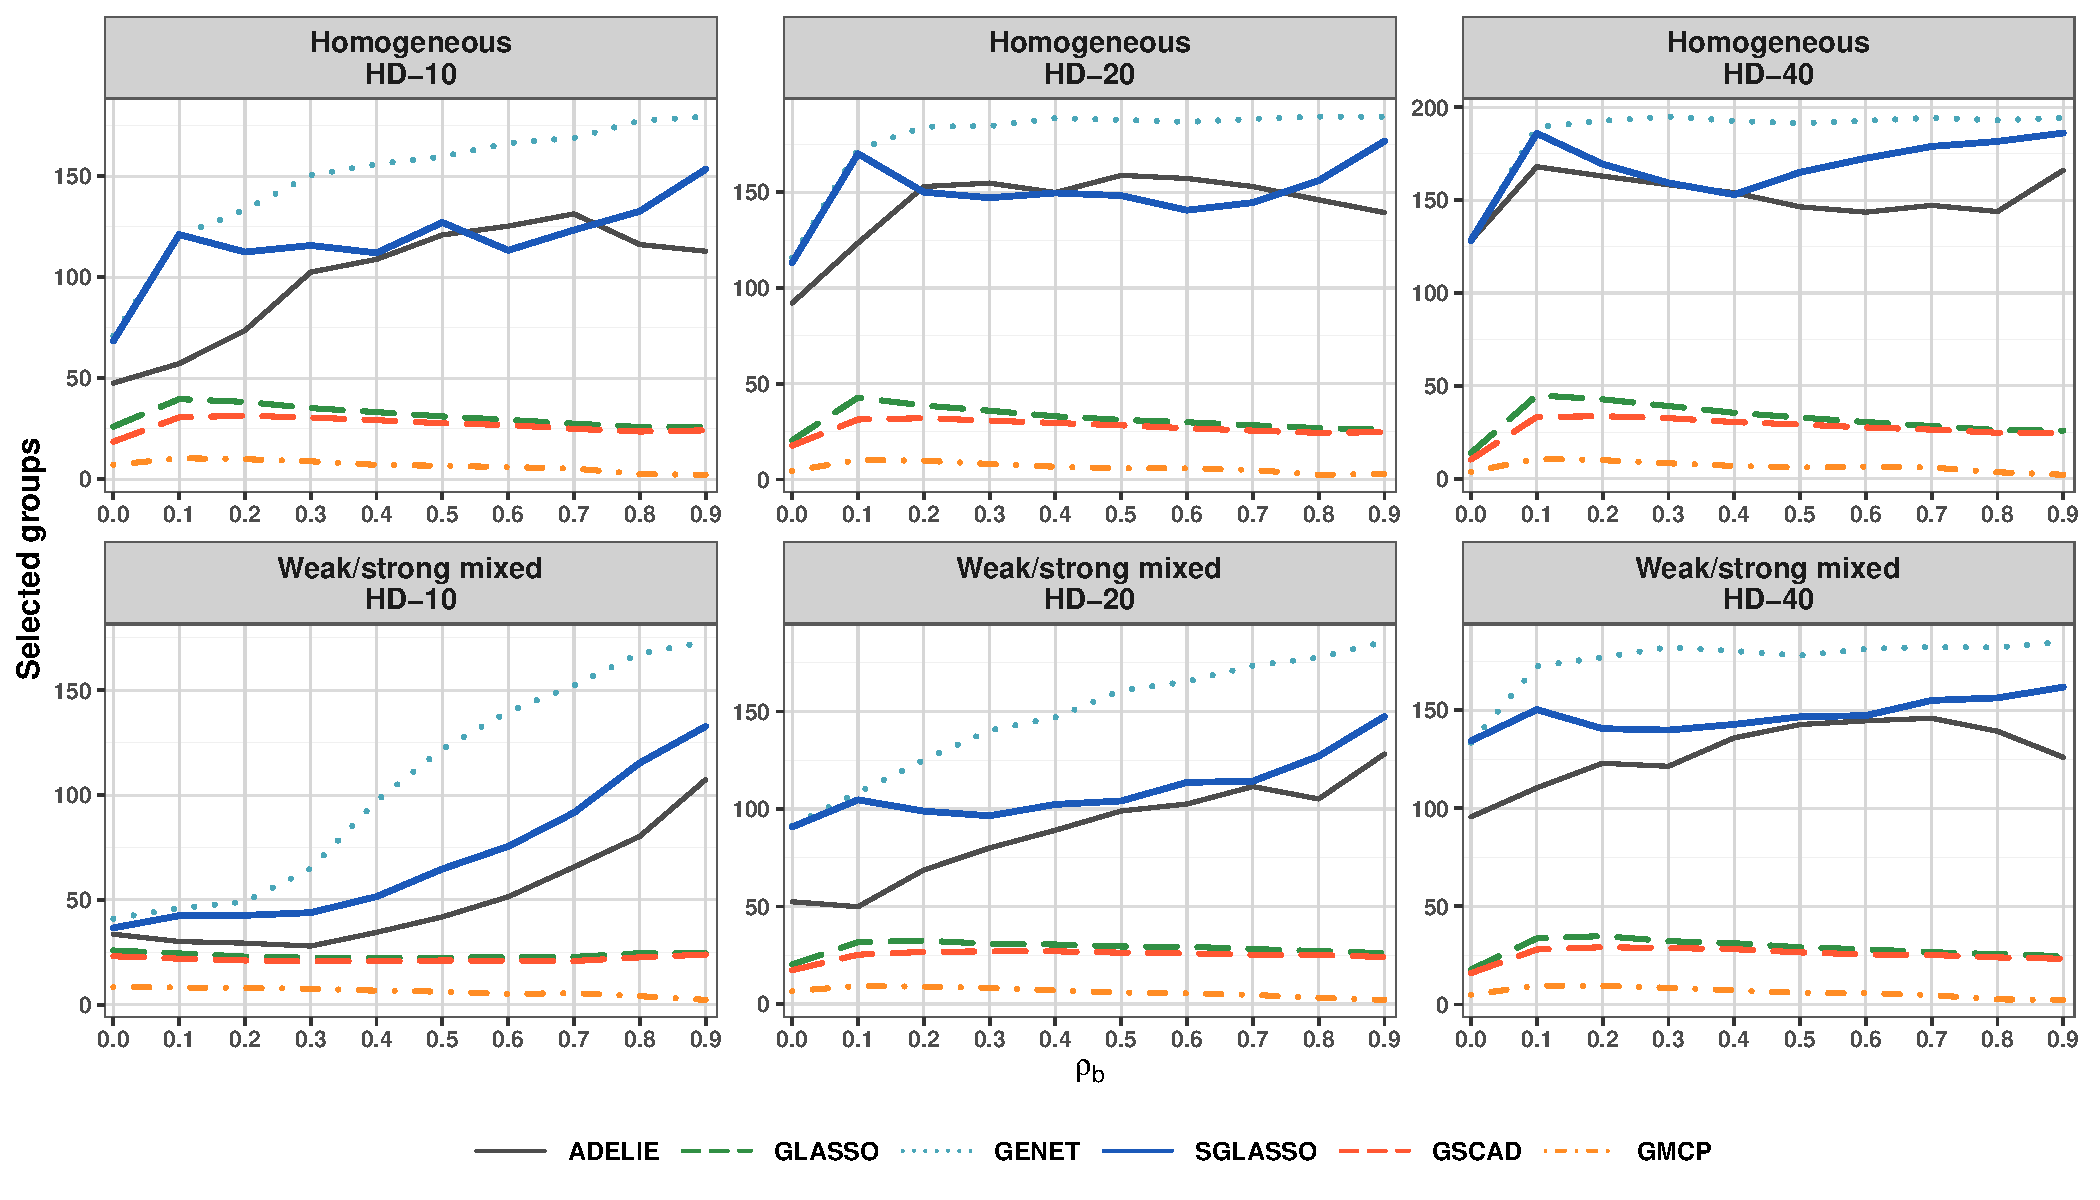
\includegraphics[width=\linewidth]{main_sim_HD_selected_groups_vs_rhob.pdf}\\[-0.25em]
\scriptsize Average number of selected groups
\end{columns}
\vspace{0.25em}
\footnotesize
SGLASSO does not target the smallest possible model. With validation-error tuning, it can select additional correlated groups when doing so improves predictive performance; FDR should therefore be interpreted jointly with test MSE and PVE.
\end{frame}

\begin{frame}{Simulation summary}
\small
\begin{columns}[T,onlytextwidth]
\column{0.48\textwidth}
\begin{block}{What is stable}
\begin{itemize}
  \item Prediction improves with stronger signal.
  \item The effect of between-group correlation is visible across all methods.
  \item SGLASSO is consistently competitive among grouped-penalty estimators.
\end{itemize}
\end{block}
\column{0.48\textwidth}
\begin{block}{What is the trade-off}
\begin{itemize}
  \item A smaller selected model is not always the best predictive model.
  \item Nonconvex group penalties can be sparse, but may lose prediction accuracy.
  \item SGLASSO often occupies an intermediate prediction-selection operating point.
\end{itemize}
\end{block}
\end{columns}
\end{frame}

\begin{frame}{Scalability among BCD solvers}
\begin{figure}
\centering
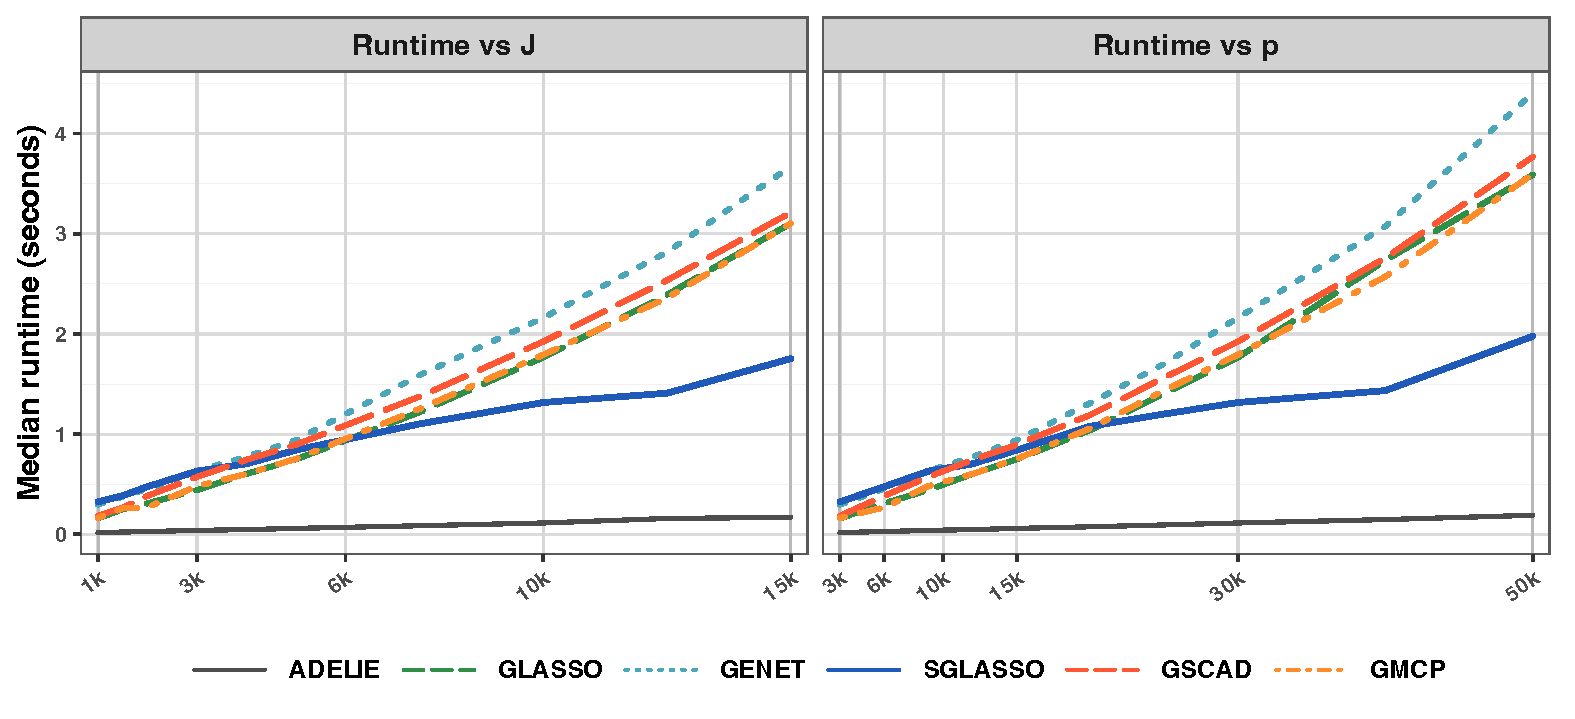
\includegraphics[width=0.98\textwidth]{runtime_scalability_curve_all_methods_linear.pdf}
\end{figure}
\vspace{-0.55em}
\footnotesize
Median serial runtime over 50 replications. ADELIE is the fastest specialized solver; SGLASSO scales favorably among BCD-type grouped-penalty methods.\par
\vspace{0.25em}
\scriptsize\color{gray}\citet{helwig2024versatile,yang2024fast}.
\end{frame}

\sectiondivider{4. Real-data application}{Gene-expression prediction with tissue and cell-type groups}

\begin{frame}{From HDDA to GenAtHum: a grouped omics problem}
\begin{columns}[T,onlytextwidth]
\column{0.53\textwidth}
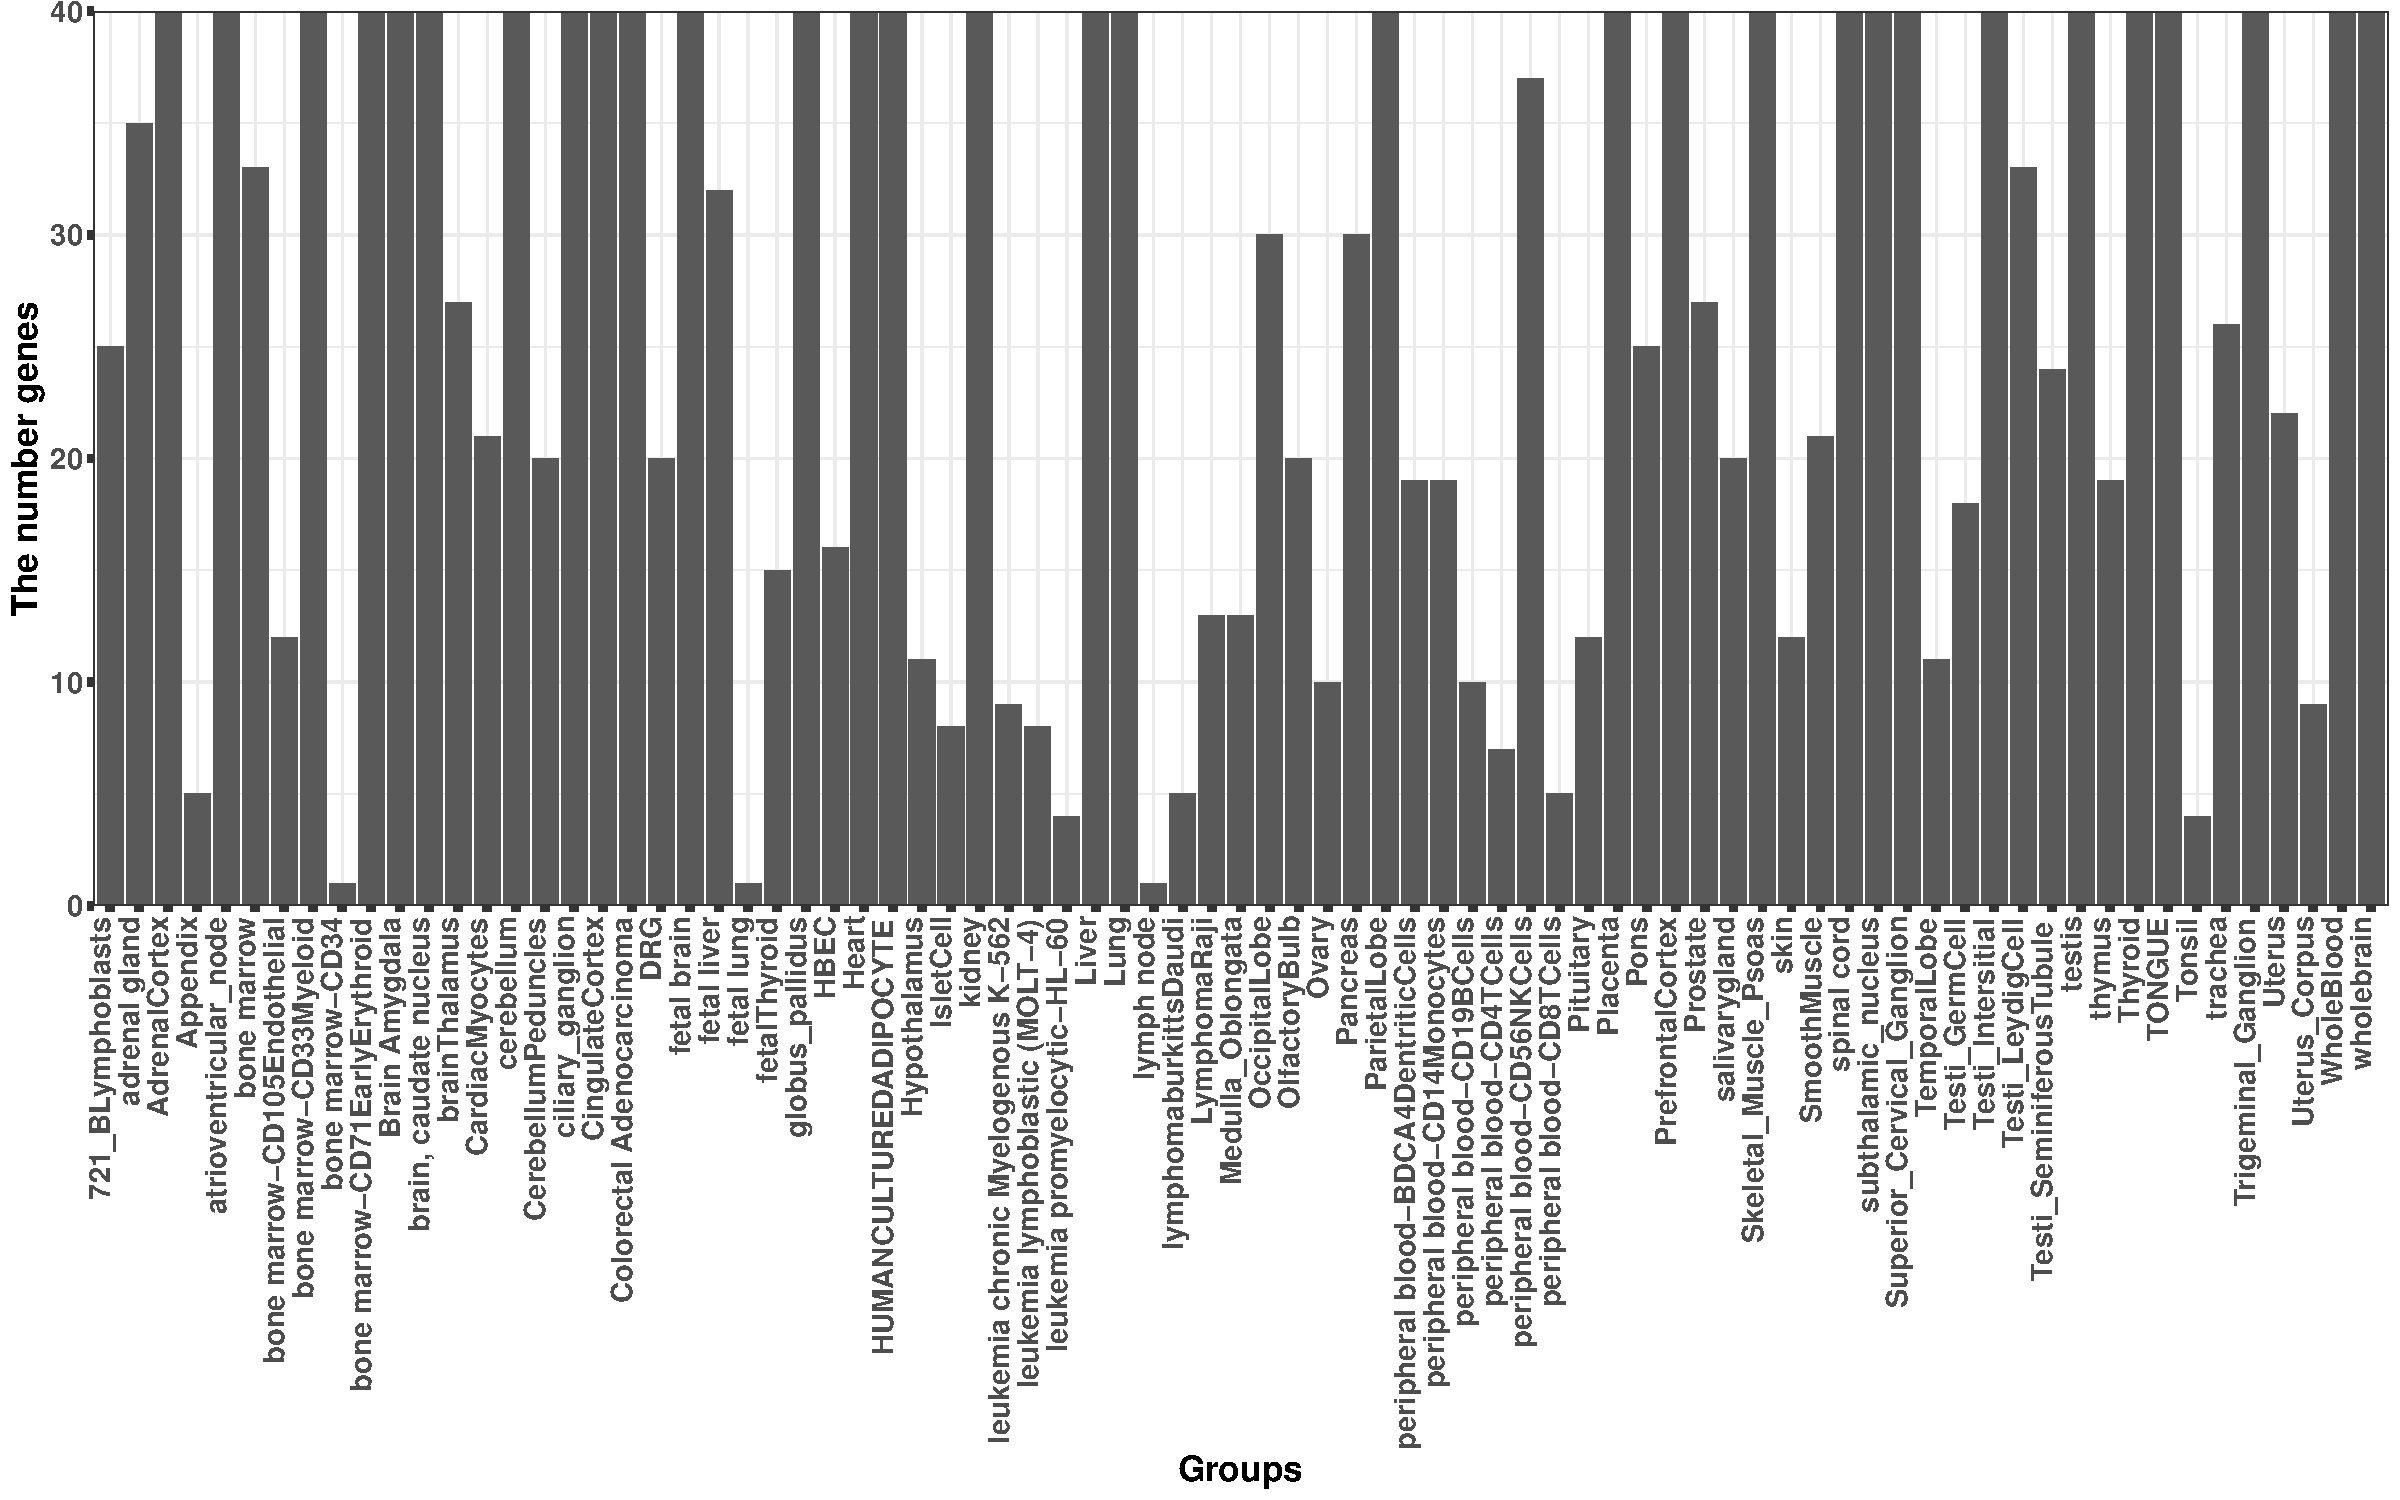
\includegraphics[height=0.48\textheight,keepaspectratio]{gene_atlas_groups.pdf}
\column{0.42\textwidth}
\scriptsize
\begin{block}{HDDA/MODAS link}
Multi-omics data combine high-dimensional measurements and biological groupings. MODAS within SABITA supports this design-to-analysis workflow.
\end{block}
\begin{block}{GenAtHum design}
$158$ samples; $2{,}045$ predictors; $79$ tissue/cell-type groups; sizes $1$--$40$. Response: MORF4L1 expression, a gene linked to DNA repair, cell-cycle, and transcriptional regulation.
\end{block}
\tiny\href{https://sabita.medipol.edu.tr/index.php/modas/}{MODAS} \textbar\
\href{https://sabita.medipol.edu.tr/}{SABITA, Istanbul Medipol University}
\end{columns}
\end{frame}

\begin{frame}{Why this real-data example is useful}
\footnotesize
\begin{columns}[T,onlytextwidth]
\column{0.48\textwidth}
\begin{block}{Statistical difficulty}
\begin{itemize}
  \item $p$ is much larger than the number of samples.
  \item Predictors are grouped by biological tissue or cell type.
  \item Correlation appears both within and across groups.
\end{itemize}
\end{block}
\column{0.48\textwidth}
\begin{block}{Scientific interpretation}
\begin{itemize}
  \item A selected group can correspond to a tissue/cell-type signal.
  \item Model size matters for interpretability.
  \item Prediction accuracy matters because the target is gene-expression prediction.
\end{itemize}
\end{block}
\end{columns}
\vspace{0.25em}
\centering\scriptsize\color{sthlmBlue}
Analysis question: can a grouped penalty improve prediction while preserving interpretable group-level structure?
\end{frame}

\begin{frame}{GenAtHum: prediction and model size}
\scriptsize
\centering
\renewcommand{\arraystretch}{1.25}
\begin{tabular}{lrrrr}
\toprule
Method & Test MSE (SE) & Relative MSE & $\widehat{s}$ & $\widehat{p}$ \\
\midrule
ADELIE  & 0.1302\;(0.0068) & 0.944 & 33 & 436.5 \\
\textbf{SGLASSO} & \textbf{0.1380\;(0.0307)} & \textbf{1.000} & \textbf{25} & \textbf{418.0} \\
GLASSO  & 0.1644\;(0.0321) & 1.191 & 12 & 89.0 \\
GENET   & 0.1652\;(0.0299) & 1.197 & 13 & 105.0 \\
GSCAD   & 0.1732\;(0.0211) & 1.255 & 10 & 84.5 \\
GMCP    & 0.1891\;(0.1043) & 1.371 & 5 & 28.0 \\
\bottomrule
\end{tabular}

\vspace{0.7em}
\begin{columns}[T,onlytextwidth]
\column{0.47\textwidth}
\begin{block}{Protocol}
Median over $100$ common 70/30 train/test splits; each training set uses 5-fold CV.
\end{block}
\column{0.47\textwidth}
\begin{block}{Reading the table}
SGLASSO has the second-smallest test MSE. Its larger selected model is consistent with prediction-focused tuning under correlated groups.
\end{block}
\end{columns}
\end{frame}

\begin{frame}{GenAtHum interpretation}
\small
\begin{columns}[T,onlytextwidth]
\column{0.47\textwidth}
\begin{block}{Prediction}
ADELIE gives the smallest median test MSE, while SGLASSO gives the second-smallest value and improves over GLASSO, GENET, GSCAD, and GMCP in this application.
\end{block}
\column{0.47\textwidth}
\begin{block}{Selection}
SGLASSO selects more predictors than GLASSO, GSCAD, and GMCP. This is not unexpected: the tuning criterion is prediction-oriented and the groups are correlated.
\end{block}
\end{columns}
\vspace{0.35em}
\begin{alertblock}{Practical reading}
For the GenAtHum data, SGLASSO behaves as a prediction-focused grouped estimator: it is not the sparsest model, but it preserves group structure and gives strong test performance.
\end{alertblock}
\end{frame}

\begin{frame}{GenAtHum: prediction with correlated gene groups}
\begin{columns}[T,onlytextwidth]
\column{0.44\textwidth}
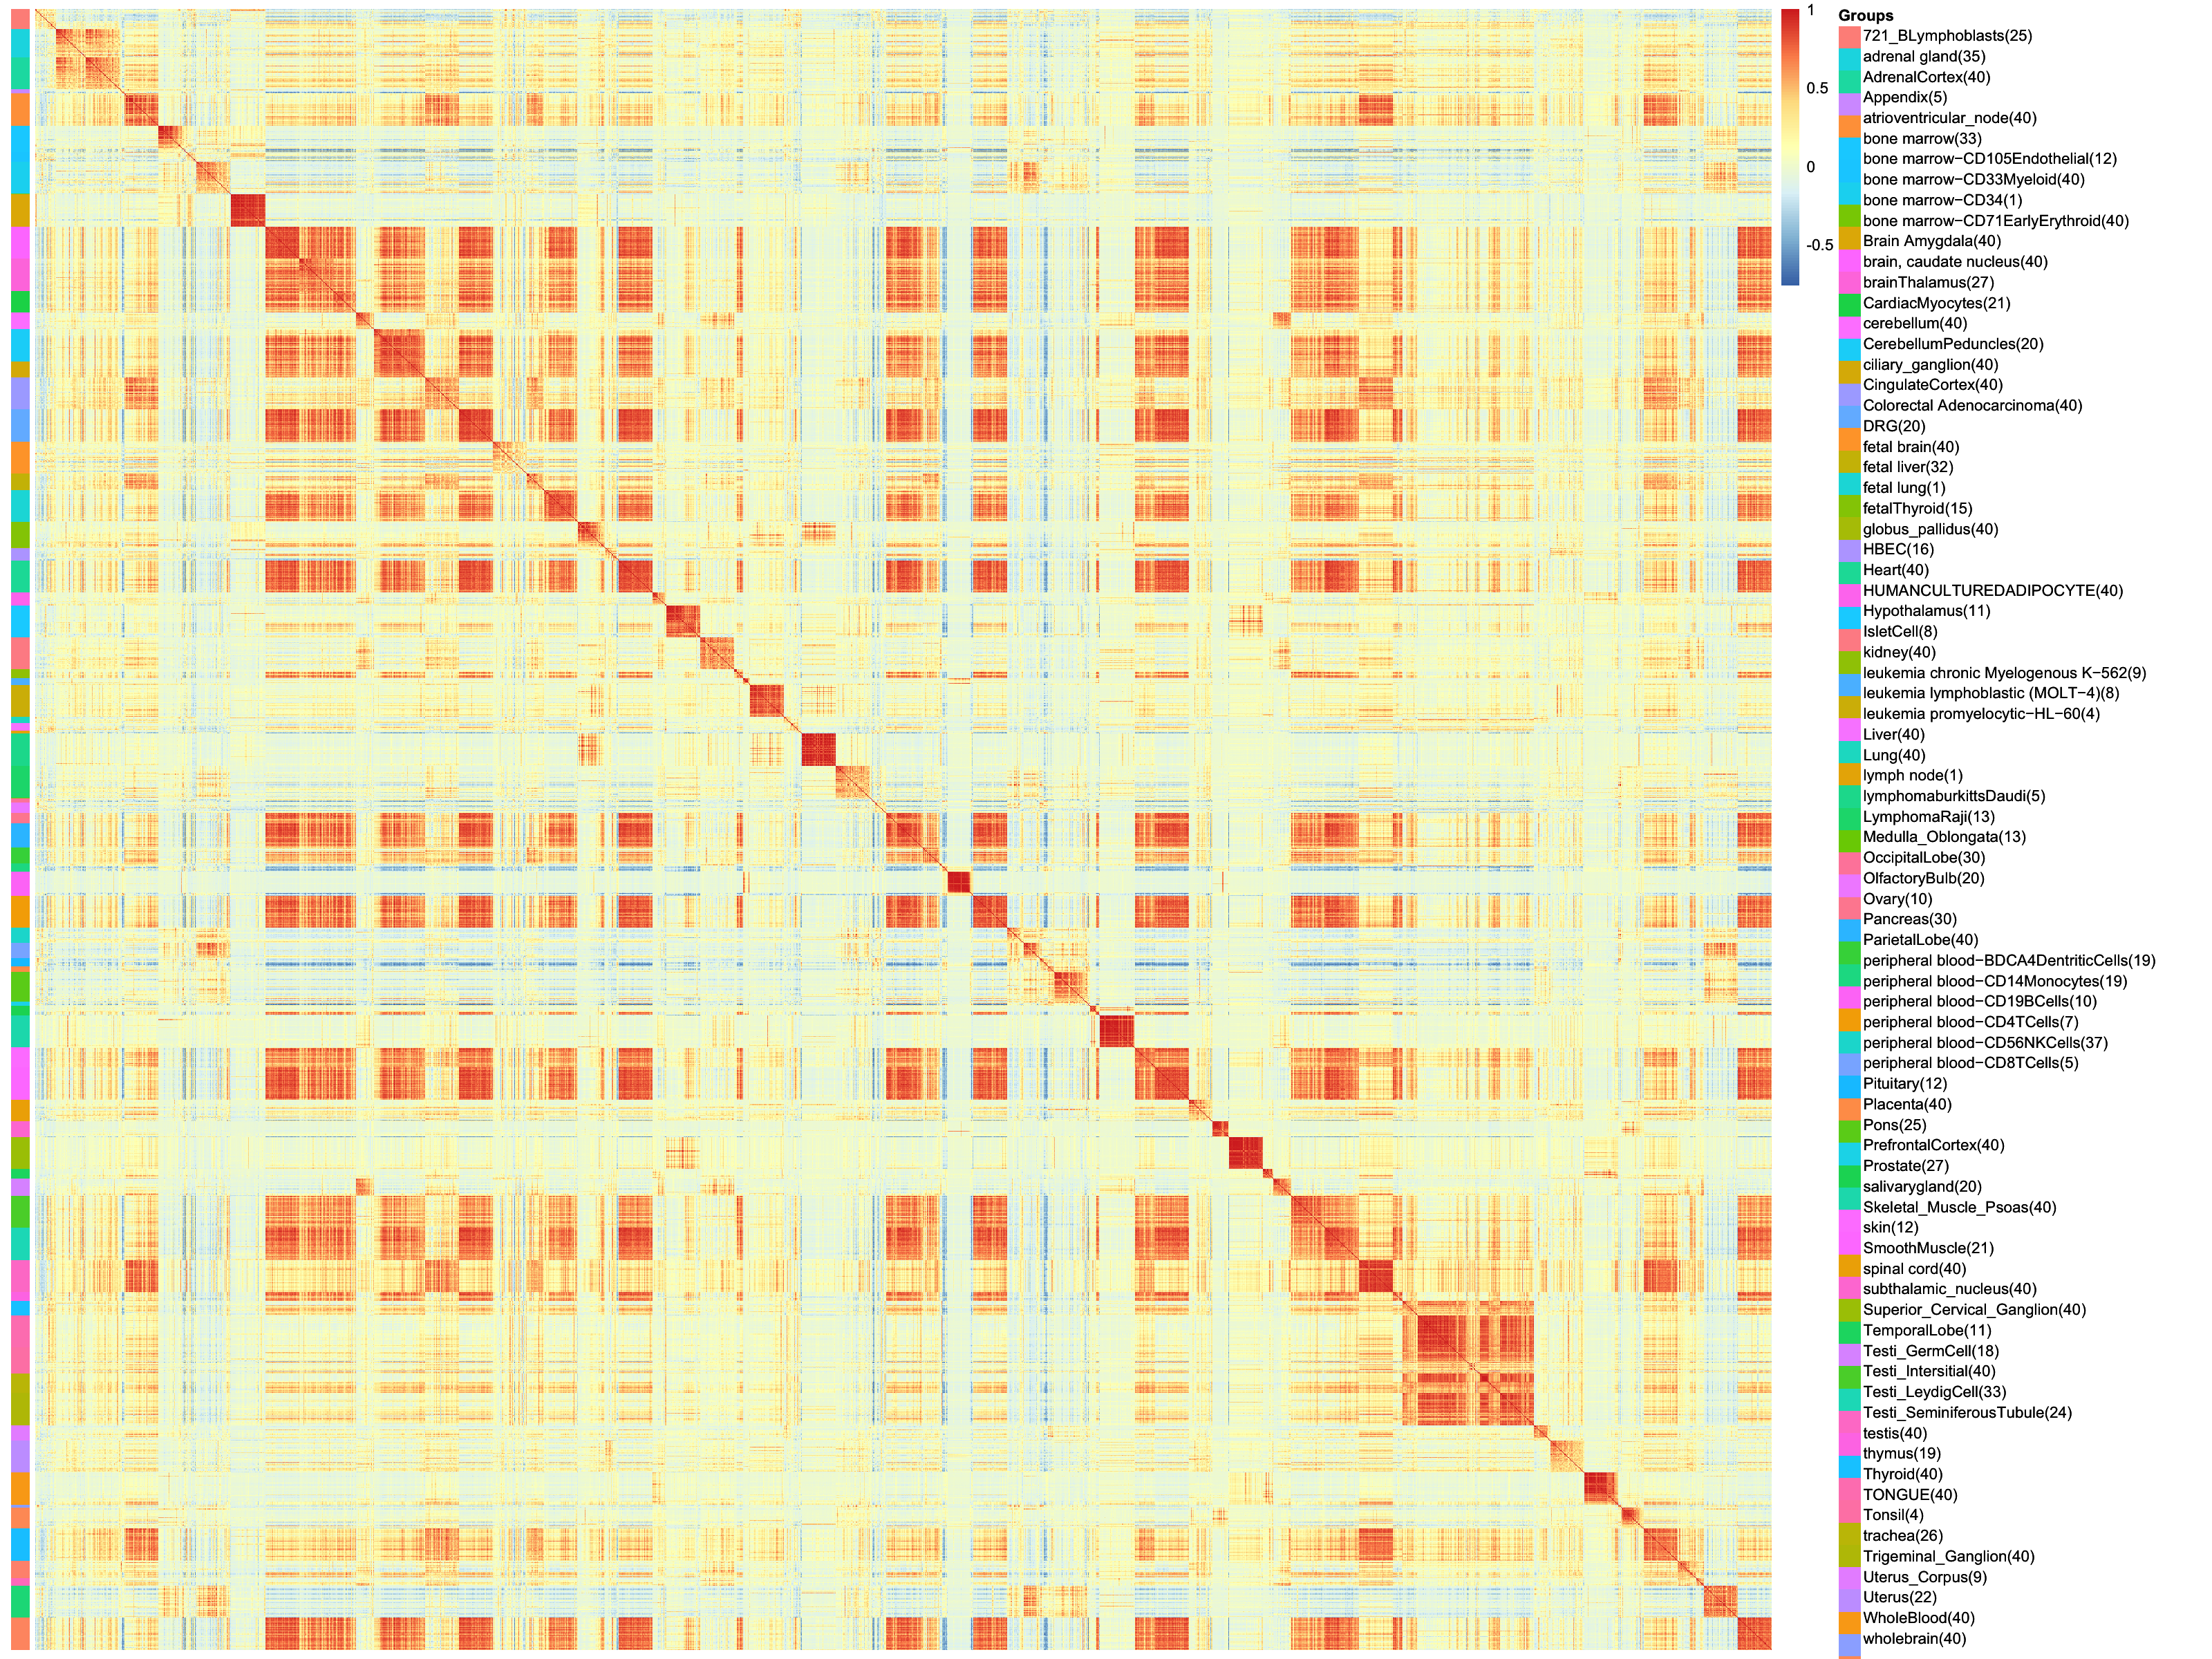
\includegraphics[width=\linewidth]{pheatmat_gene.png}
\column{0.51\textwidth}
\scriptsize
\begin{block}{Evaluation protocol}
$100$ repeated 70/30 train/test splits; identical splits and 5-fold CV for every method.
\end{block}
\begin{block}{SGLASSO result}
Median test MSE: $0.1380$. Median model: $25$ groups and $418$ predictors.
\end{block}
\begin{exampleblock}{Interpretation}
Second-smallest test MSE after ADELIE; lower MSE than GLASSO, GENET, GSCAD, and GMCP.
\end{exampleblock}
\end{columns}
\end{frame}

\begin{frame}{Cross-validation paths}
\begin{figure}
\centering
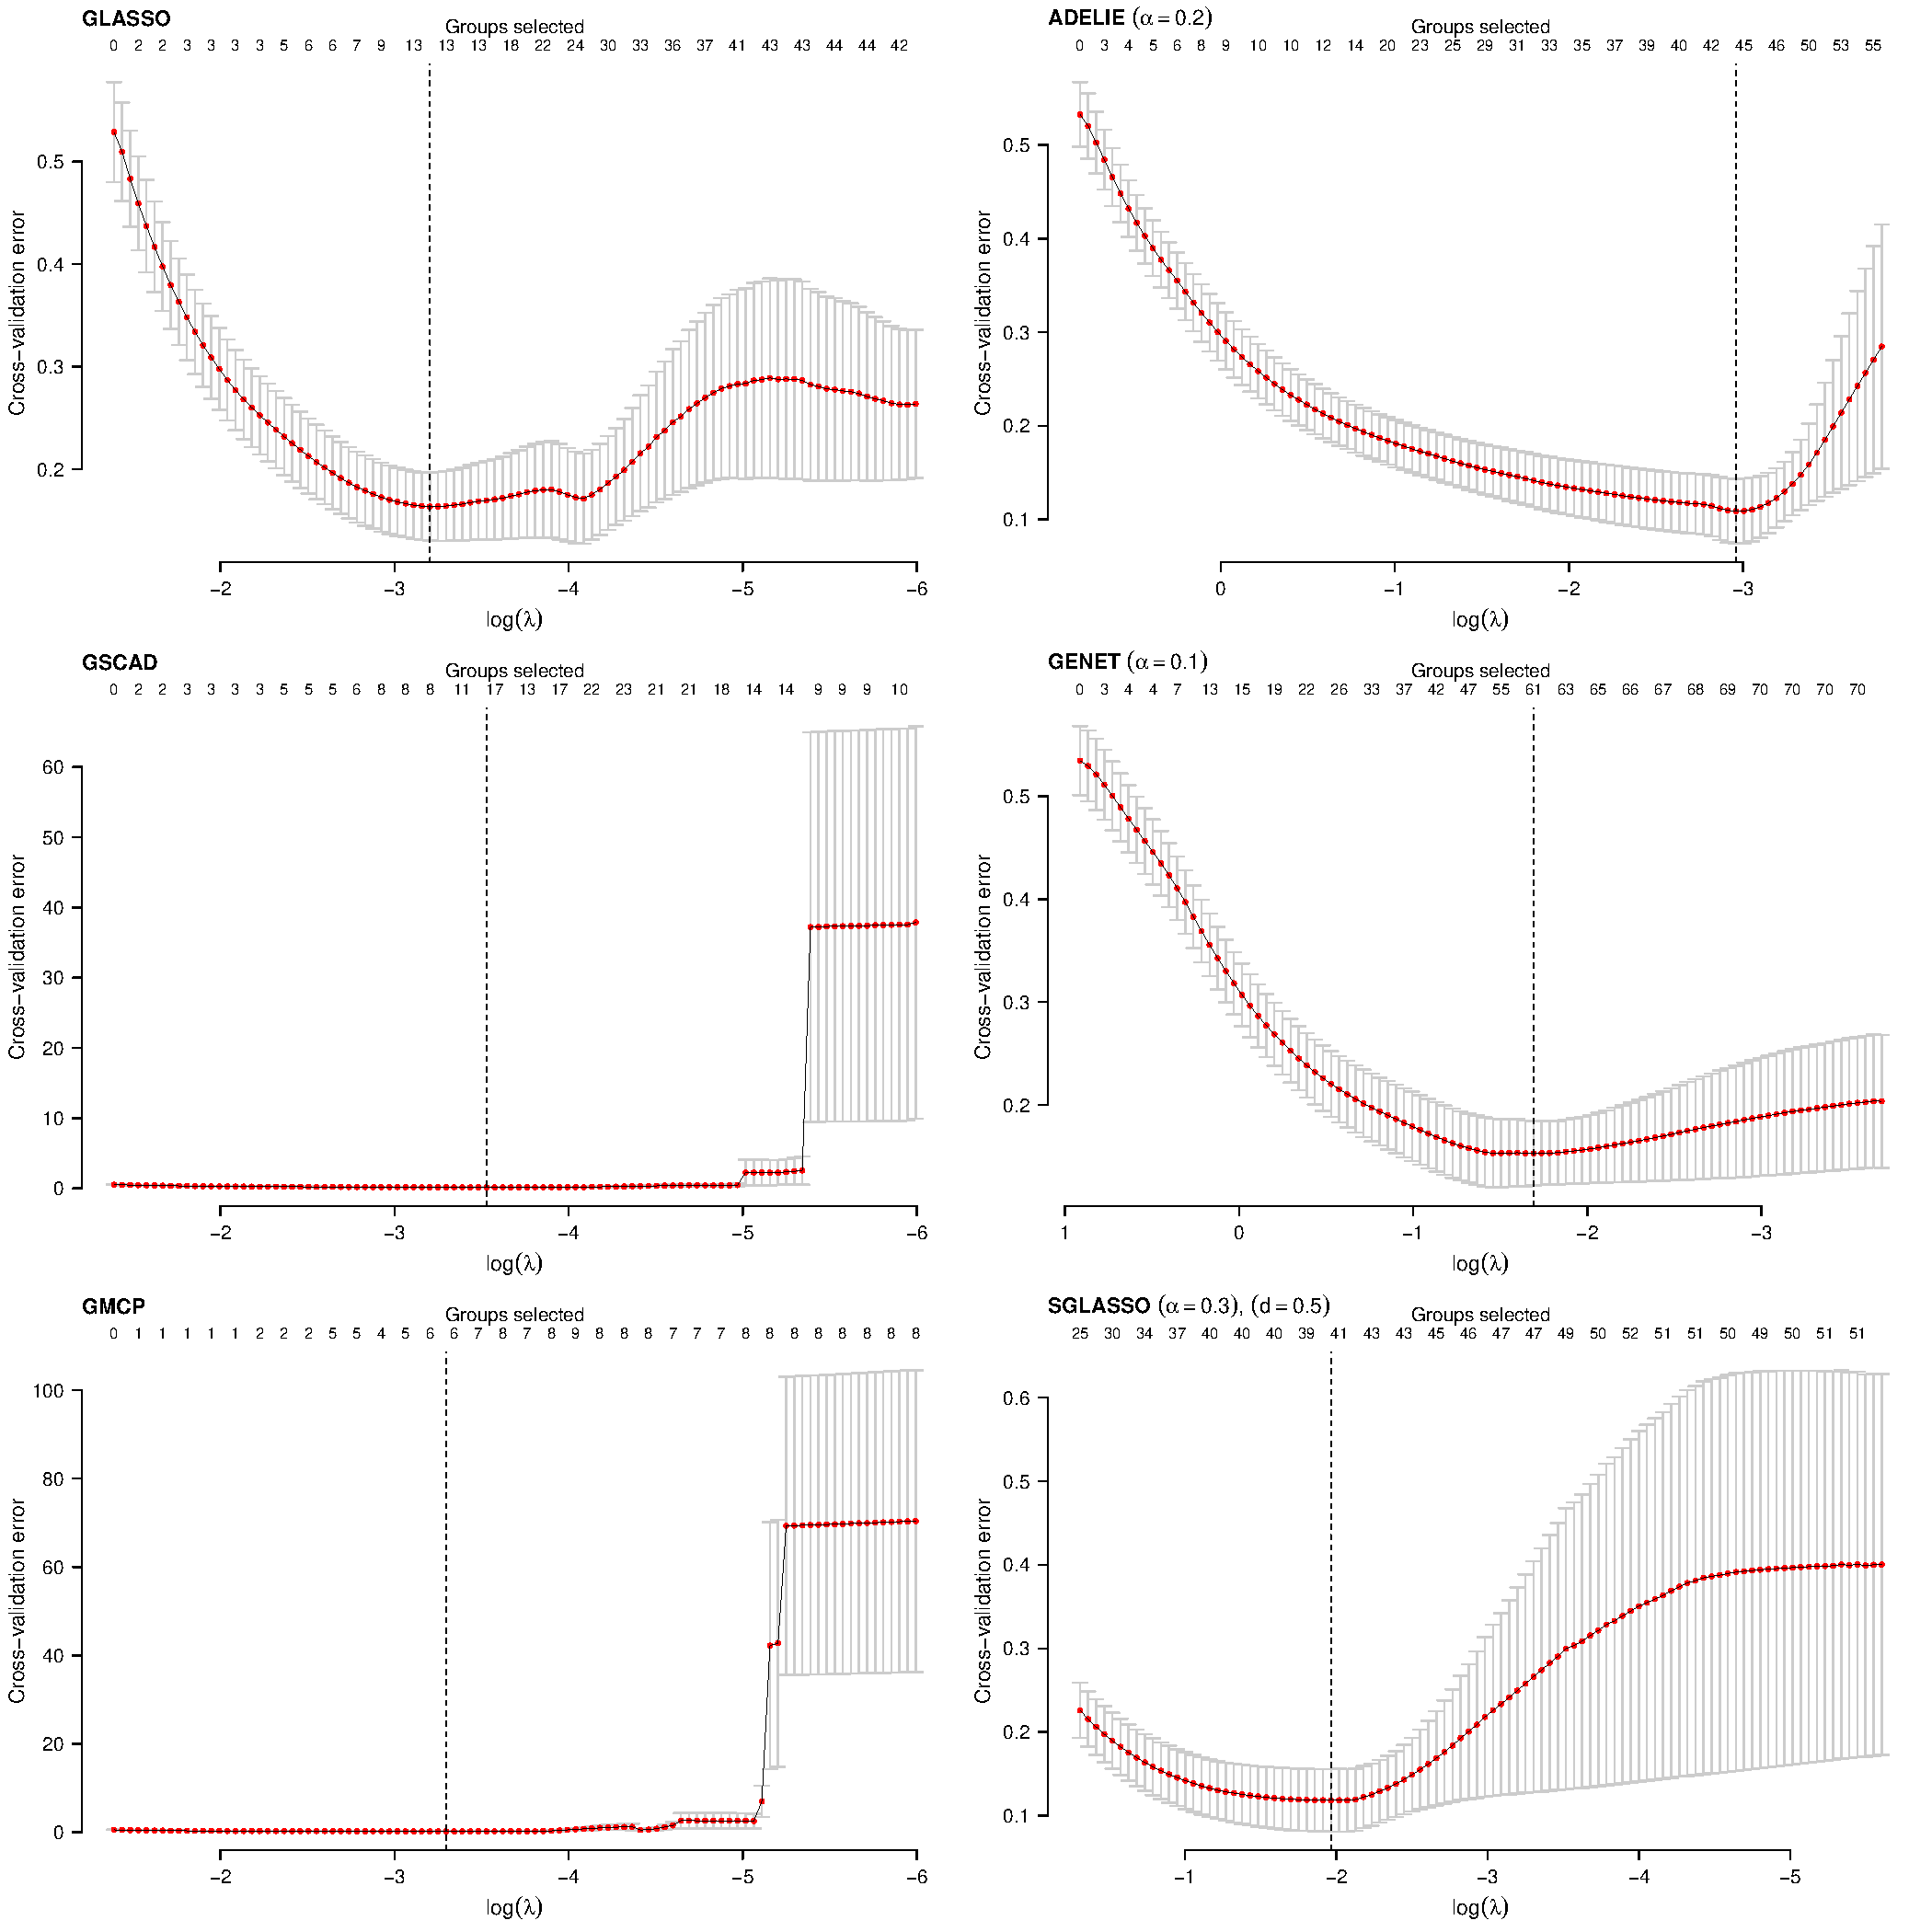
\includegraphics[height=0.61\textheight,keepaspectratio]{CV_Plots_GenAtHum.pdf}
\end{figure}
\vspace{-0.8em}
\footnotesize
Full-data 5-fold CV across six methods. SGLASSO can retain a broader correlated model when this improves CV prediction.
\end{frame}

\sectiondivider{5. Take-home message}{A flexible groupwise operating point for correlated high-dimensional data}

\begin{frame}{What SGLASSO contributes}
\small
\begin{enumerate}
  \item \textbf{A flexible groupwise target:} combines selection with scaled shrinkage toward a least-squares-based target.
  \item \textbf{A practical solver:} BCD, warm starts, sequential screening, residual updates, and KKT verification.
  \item \textbf{A complementary operating point:} competitive prediction and estimation under correlated groups, with sparsity controlled by the tuning criterion.
\end{enumerate}

\vspace{0.5em}
\begin{alertblock}{Take-home message}
For overlapping or heterogeneous correlated signal, the best predictive model need not be the smallest one. SGLASSO tunes that trade-off.
\end{alertblock}
\end{frame}

\begin{frame}{When would I use SGLASSO?}
\small
\begin{columns}[T,onlytextwidth]
\column{0.48\textwidth}
\begin{block}{Use it when}
\begin{itemize}
  \item groups are scientifically meaningful;
  \item predictors are correlated within or across groups;
  \item prediction and group-level interpretation both matter;
  \item zero-centered shrinkage may be too restrictive.
\end{itemize}
\end{block}
\column{0.48\textwidth}
\begin{block}{Interpret results as}
\begin{itemize}
  \item a selected set of predictive groups;
  \item a regularized coefficient path;
  \item a trade-off among test error, coefficient recovery, and sparsity;
  \item not merely a minimum-FDR procedure.
\end{itemize}
\end{block}
\end{columns}
\end{frame}

\begin{frame}{Limitations and next steps}
\footnotesize
\begin{columns}[T,onlytextwidth]
\column{0.48\textwidth}
\begin{block}{Current scope}
\begin{itemize}
  \item Linear Gaussian grouped regression.
  \item Known, non-overlapping groups.
  \item Tuning by validation, information criteria, or cross-validation.
\end{itemize}
\end{block}
\column{0.48\textwidth}
\begin{block}{Natural extensions}
\begin{itemize}
  \item Generalized linear models.
  \item Overlapping or hierarchical groups.
  \item Faster second-order block updates for very large grouped designs.
\end{itemize}
\end{block}
\end{columns}
\vspace{0.25em}
\centering\scriptsize\color{sthlmBlue}
Closing point: SGLASSO adds a flexible grouped-regularization option when collinearity makes the prediction-selection trade-off visible.
\end{frame}

\begin{frame}{Research context and support}
\footnotesize
\begin{columns}[T,onlytextwidth]
\column{0.48\textwidth}
\begin{block}{Research setting}
\begin{itemize}
  \item Developed during postdoctoral research at Simon Fraser University, Canada.
  \item Supported by the T\"{U}B\.{I}TAK B\.{I}DEB 2219 programme.
\end{itemize}
\end{block}
\column{0.48\textwidth}
\begin{block}{Computing and dissemination}
\begin{itemize}
  \item Large simulation experiments were run on the T\"{U}B\.{I}TAK ULAKB\.{I}M TRUBA infrastructure.
  \item Published in \emph{The American Statistician} (2026).
\end{itemize}
\end{block}
\end{columns}
\vspace{0.4em}
\begin{alertblock}{Resources}
\href{https://doi.org/10.1080/00031305.2026.2709494}{Published article: \emph{The American Statistician}} \qquad
\href{https://github.com/byuzbasi/sglasso}{GitHub: \pkg{sglasso}}
\end{alertblock}
\end{frame}

\begin{frame}{Selected references}
\tiny
\bibliographystyle{plainnat}
\bibliography{references}
\end{frame}

\begin{frame}{Thank you}
\Large
\textbf{Package and reproducible code}\\[0.5em]
\normalsize
\url{https://github.com/byuzbasi/sglasso}

\vspace{1.25em}
\textbf{Contact}\\[0.5em]
\normalsize
Bahad{\i}r Y\"{u}zba\c{s}{\i}\\
\.{I}n\"{o}n\"{u} University
\end{frame}

\end{document}
